% ============================================================
% Understanding the Great Stagnation
% Draft of 2026-11-16: complete. Every model number between THEORY-NUMBERS-BEGIN and THEORY-NUMBERS-END is
% recomputed by checks/check_theory.py (group Q) from code/model.py; every number between DATA-NUMBERS-BEGIN and
% DATA-NUMBERS-END (the abstract, the introduction, Sections 5-7) by checks/check_data.py from the cached pulls and
% the measurement scripts (code/m1_eras.py ... m5_recent.py, hx_test.py); Table B.1 is written by
% code/table_regimes.py. Journal references were checked against Crossref on 2026-11-16.
% ============================================================
\documentclass[12pt]{article}
\usepackage[T1]{fontenc}
\usepackage{lmodern}
\usepackage[utf8]{inputenc}
\usepackage[a4paper, margin=2.5cm]{geometry}
\usepackage{setspace}
\onehalfspacing
\clubpenalty=10000
\widowpenalty=10000
\usepackage{amsmath, amssymb, amsthm}
\usepackage{bm}
\usepackage{graphicx}
\usepackage{booktabs}
\usepackage{array}
\usepackage[labelfont=bf, labelsep=period, font={footnotesize,stretch=1}, justification=justified]{caption}
\usepackage{microtype}
\usepackage{titlesec}
\usepackage{xcolor}
\usepackage[hidelinks]{hyperref}

\theoremstyle{plain}
\newtheorem{proposition}{Proposition}
\newtheorem{lemma}{Lemma}

\newcommand{\refentry}[1]{\par\hangindent=1.5em\hangafter=1\noindent #1}
\newcommand{\draftnote}[1]{\par\smallskip\noindent\colorbox{black!6}{\parbox{\dimexpr\linewidth-2\fboxsep\relax}{%
  \footnotesize\itshape Draft note. #1}}\par\smallskip}

\title{\bfseries Understanding the Great Stagnation\thanks{Views are the author's own and do not represent those of
  KTH or SEB. Prepared with Claude (Anthropic); see the declaration on generative AI at the end.}\\[7pt]
  \large\mdseries Machine progress, scarce land, and the hours that did not fall}
\author{Stella Wilson\thanks{KTH Royal Institute of Technology and Skandinaviska Enskilda Banken (SEB). Email:
  \texttt{thmwi@kth.se}.}}
\date{Draft, November 2026}

\begin{document}
\maketitle

% DATA-NUMBERS-BEGIN
\begin{abstract}
\noindent Since the early 1970s, and again since the mid-2000s, U.S. output per hour has grown slowly while machines, computers above all, improved fast. We argue that measured productivity is an equilibrium outcome: the inverse of the hours an economy uses per unit of output. In a task economy whose prices resolve into hours and the rents of inputs that cannot be produced, and in which people need land in fixed proportion to goods, land caps output. Hours that cannot leave work are re-employed at tasks where machines are relatively better, so output per hour falls with technology unchanged. As machines improve, the wage relative to rent and labor's share tend to zero, and output per hour converges to a ceiling, land per remaining hour over land per basket, unless support outside work is funded and unconditional. A lower required return on capital also lowers the wage relative to rent and labor's share. In U.S. data, by criteria written down before the data were pulled, the shift of output toward slow sectors and the reallocation of hours account for 47 and 38 percent of the slowdowns of 1973--95 and 2004--19 against 1948--73, though 27 and 19 percent without the end of the farm exodus, a reading added afterwards; shelter accounts for about a third of the rise of consumer relative to producer prices that makes up most of the gap between pay and productivity. A pre-registered cross-country test of absorption is uninformative.
\end{abstract}

\noindent\textbf{Keywords:} productivity slowdown; automation; land rent; labor force participation; disguised unemployment; secular stagnation; task models\\
\textbf{JEL codes:} O47, O33, E24, J22, R31, E43

\section{Introduction}\label{sec:1}

Output per hour in the U.S. nonfarm business sector grew 2.8 percent a year between 1948 and 1973. It grew 1.4 percent a year between 1973 and 1995 and, after a decade of 3.0 percent during the spread of information technology, 1.5 percent a year between 2004 and 2019. Over the same decades the cost of computation fell by many orders of magnitude (Nordhaus 2007). Solow (1987) put the puzzle in one line: the computer age could be seen everywhere but in the productivity statistics.

The slowdown came with other changes that are usually studied apart. On decade averages, labor's share of income in the nonfarm business sector was 9.3 percent lower in 2016--25 than in the 1990s, after falling 3.6 percent between 1948--57 and the 1990s. Average hours per worker in the United States, which fell 0.31 percent a year between 1950 and 1980, have fallen 0.07 percent a year since, half a century after Keynes (1930) expected his grandchildren to work fifteen hours a week. The ten-year real interest rate fell from 6.5 percent in 1982--84 to below zero in 2020. Land, rather than structures, accounts for a growing share of the value of housing (Davis and Heathcote 2007; Knoll, Schularick, and Steger 2017): 22 percent of the value of households' owner-occupied real estate in 1952--72 and 37 percent in 2004--19. Much of the rise in the capital share is housing (Rognlie 2015). Deflated by the consumer prices of durable goods and of shelter, the same hourly wage diverged by a factor of 4.8 between 1964 and 2024 (B\r{a}ge and Wilson 2026).

Existing accounts read these facts as separate puzzles, or as signs of one shortage: of ideas (Gordon 2016; Cowen 2011; Bloom, Jones, Van Reenen, and Webb 2020), of demand (Summers 2014; Mian, Straub, and Sufi 2021), or of competition (De Loecker, Eeckhout, and Unger 2020; Philippon 2019). Section~\ref{sec:2} reviews them. We propose an account in which they come from one cost system, moved by a few primitives: machine capability, the return required on capital, and who can leave work. In it, slow growth of measured productivity is not evidence that machines stopped improving.

Output per hour is a ratio of two equilibrium quantities. In a task economy, where firms assign each task to whichever of labor and machines performs it more cheaply (Zeira 1998; Acemoglu and Restrepo 2018), the hours used per unit of output depend on where the line between machine and human tasks sits, and that line depends on how many hours people offer. If more people must work at any wage, the wage falls until firms take them on, at tasks where machines are relatively better than at the tasks labor already holds. The hours used per unit of output rise and output per hour falls, with technology unchanged. Robinson (1936) called the re-employment of displaced workers in occupations of lower productivity disguised unemployment. A version of it, spread over decades, is what we think the great stagnation looks like from inside the productivity statistics.

Who must work at any wage? People whose consumption is financed by their own wages and who have no support if they leave work; people whose support is paid only when they work; and people whose support has been eaten by the rents of the land and the other inputs that support requires. B\r{a}ge and Wilson (2026) price the machine that replaces a worker and the living basket that sustains a person outside work through one cost system, in which every price resolves into hours and the rents of inputs that cannot be produced. We take their stationary economy, with durable machines and land, and generalize who can leave work: a share $\theta$ of people has no support outside work, the rest have a basket of support in work and out, and support can include a payment $\Delta$ for working.

Three results follow. First (Proposition~\ref{prop:1}), when $\theta$ or $\Delta$ rises, the line moves toward labor: hours and output rise, and output per hour, the wage relative to rent and the wage in baskets all fall. In an instance whose parameters were set from U.S. cost shares, output per hour is 26 percent lower when nobody can leave work than when everyone can, with the same machines. Second (Proposition~\ref{prop:2}), as machines improve at every task, output converges to the land endowment over land per basket under every rule, and the wage relative to rent and labor's share tend to zero: income moves to the owners of land. What the rules decide is the hours. When some hours cannot fall, output per hour converges to a ceiling, land per remaining hour divided by land per basket, which machine progress cannot raise, and its elasticity with respect to machine capability goes to zero. When exit is funded and unconditional, hours fall toward zero and output per hour eventually rises in proportion to machine capability. Third (Proposition~\ref{prop:3}), a lower required return on capital cheapens machine services relative to land. Whoever can leave work, it lowers the wage relative to rent and labor's share, and raises the price of land in hours of work; at a given threshold, the elasticity of the wage--rent ratio with respect to the user-cost rate is the inverse of land's share of a machine's cost. It raises output per hour only where people can leave work. Two lemmas connect these results to measured prices. The ratio of real pay to output per hour is labor's share times the ratio of producer to consumer prices, and the price ratio falls with the wage--rent ratio when consumption is more land-intensive than measured output, counted along the chains that set prices (Lemma~\ref{lem:2}). With an elasticity of substitution below one between machine-made goods and goods bound by land or by people, measured growth converges to the bound goods' growth (Lemma~\ref{lem:3}; Baumol 1967).

The account does not claim that the technological frontier failed to slow: the industries that produce computers slowed after 2004 too (Fernald 2015). It claims that the measured aggregate can stall while machines improve, and it says what must hold for that to happen: some hours cannot fall, and some goods need land or people in proportions that machine progress cannot change. 
Section~\ref{sec:5} measures the account's implications, with each prediction and what would count against it written down before the data were pulled. In U.S. industry data, the shift of value added toward slow sectors and the reallocation of hours account for 47 percent of the slowdown of 1973--95 against 1948--73 and 38 percent of that of 2004--19, which the criterion written beforehand reads as support; much of it is the end of the movement of hours out of agriculture: without agriculture, a reading added after the data were seen, the shares are 27 and 19 percent. Composition took even more from the growth of 1995--2004, so what separates the slow eras from the boom lies within sectors. The rise of consumer relative to producer prices makes up 73 percent of the gap between pay and productivity since 1973, and shelter accounts for 37 percent of that rise. Had U.S. hours per worker kept falling after 1980 at their pace of 1950--80, output per hour would, at given technology and the model's elasticity, have been 6.5 percent higher in 2023, or 0.15 points a year. Since 2019 output per hour has grown faster as hours per person fell and the pay of production and nonsupervisory employees rose relative to the average. The cross-country test, fixed in every detail before its data were pulled, is uninformative: across OECD countries, faster growth of hours went with faster growth of output per hour, though not significantly, and within countries, over five-year periods, with slower growth. Section~\ref{sec:6} collects the predictions and what the measurements say about the rivals.

Section~\ref{sec:3} sets out the model and Section~\ref{sec:4} the results, which Appendix~\ref{app:A} proves; Appendix~\ref{app:B} reports the instance and the checks, and Appendix~\ref{app:C} the record of the plan. Section~\ref{sec:7} concludes with policy and artificial intelligence.
% DATA-NUMBERS-END

\section{Accounts of the great stagnation}\label{sec:2}

\textbf{Exhausted opportunities.} Gordon (2016) argues that the great inventions of 1870--1970 transformed living standards once, that the inventions since are narrower, and that demography, education, inequality and debt add headwinds. Cowen (2011) argues that the United States had used up its low-hanging fruit, free land among it. Bloom, Jones, Van Reenen, and Webb (2020) find that research productivity has fallen across fields: sustaining a constant rate of progress takes ever more researchers. These accounts locate the slowdown in the rate at which technology improves. Ours does not need that rate to fall.

\textbf{Energy.} The slowdown began with the oil shock of 1973. Bruno and Sachs (1985) explain the stagflation that followed by shocks to the supply of energy and raw materials meeting rigid wages, and Jorgenson (1988) traces much of the slowdown of productivity growth in U.S. industries to higher energy prices. A deposit of oil is a non-produced input in the accounting used here, as a site is; Section~\ref{sec:6} compares the two in the price data.

\textbf{Measurement.} If price indexes overstate inflation for new and free digital goods, real growth is understated. Byrne, Fernald, and Reinsdorf (2016) and Syverson (2017) conclude that mismeasurement cannot account for the size and timing of the slowdown. We take measured output as given.

\textbf{Labor's share.} Karabarbounis and Neiman (2014) attribute much of the global fall in labor's share to the falling relative price of investment goods, a channel close to Proposition~\ref{prop:3}'s, in which cheaper machine services lower the wage relative to rent. Elsby, Hobijn, and \c{S}ahin (2013) point to the measurement of the self-employed's income and to offshoring, and Autor and Salomons (2018) to productivity growth within industries; Gutiérrez and Piton (2020) find that, outside housing, the fall is concentrated in the United States.

\textbf{Demand and the interest rate.} Hansen (1939) argued that slower population growth and the closing of the frontier would leave investment short of saving. Summers (2014) revived the argument as secular stagnation, a natural rate of interest too low for monetary policy to reach; Eggertsson, Mehrotra, and Robbins (2019) give it a quantitative model, and Mian, Straub, and Sufi (2021) trace low rates to saving by the rich lent to everyone else. In those accounts low rates are a symptom of weak demand. Here a lower required return is also a force on the supply side: it cheapens machine services relative to land, lowers the wage relative to rent, and raises the price of land in hours of work (Proposition~\ref{prop:3}).

\textbf{Market power.} De Loecker, Eeckhout, and Unger (2020) document rising markups since 1980, and Philippon (2019) a decline of competition in U.S. markets. In the accounting used here, markups sustained by exclusion are institutional rents: income accruing to an input whose supply production does not expand, like the rent of land.

\textbf{Structural change.} Baumol (1967) showed that when the relative prices of slow-productivity services rise and demand for them is inelastic, they take a growing share of spending and slow aggregate growth; Nordhaus (2008) studies the effect in U.S. industry data, and Ngai and Pissarides (2007) give the multisector growth model. Vollrath (2020) reads the slowdown as a by-product of success: the shift to services and slower population growth. Comin, Lashkari, and Mestieri (2021) find that income effects drive most of the shift toward services, and Borri and Reichlin (2018) apply Baumol's argument to housing, whose construction lags in productivity. Lemma~\ref{lem:3} is the version of Baumol's result in which goods are bound by land or by tasks only people can do.

\textbf{Land and housing.} Ricardo (1817) and George (1879) held that the gains from progress go in the end to the owners of land. Rising house prices are largely rising land prices (Davis and Heathcote 2007; Knoll, Schularick, and Steger 2017), and much of the rise in the capital share is housing (Rognlie 2015). Glaeser and Gyourko (2018) trace high housing costs to limits on building. Hsieh and Moretti (2019) estimated large output losses from housing constraints in productive cities; Greaney (2026) finds errors in that computation and a far smaller effect. Goolsbee and Syverson (2023) document falling productivity in U.S. construction. In our account land matters less through where people can afford to live than through the ceiling it puts on output per hour when hours cannot fall (Proposition~\ref{prop:2}).

\textbf{Hours, employment, and productivity.} Keynes (1930) expected rising productivity to shorten the working week to fifteen hours. Robinson (1936) observed that workers displaced in a slump take up occupations of lower productivity rather than remaining idle; Lewis (1954) built a theory of development on labor held at low productivity. Across European countries, Dew-Becker and Gordon (2012) find that employment growth after the labor-market reforms of the late 1990s came with slower productivity growth, and Bourl\`es and Cette (2007) adjust productivity levels for the hours and employment rates behind them. Boppart and Krusell (2020) find that hours per worker have fallen steadily as productivity grew, across countries and over a century, and write preferences under which they fall at a constant rate along balanced growth. Acemoglu, Autor, Dorn, Hanson, and Price (2014) find that the productivity gains of U.S. manufacturing industries that use information technology intensively came with falling employment rather than rising output. Prescott (2004) attributes lower European hours to taxes on labor, and Warren and Tyagi (2003) argue that second incomes in American families were bid into the price of housing. Habakkuk (1962) and Allen (2009) argue that dear labor induced mechanization, and Acemoglu (2010) states when labor scarcity encourages innovation. Proposition~\ref{prop:1} gives the mechanism behind the trade-off between employment and productivity in a cost system with land.

\textbf{Wages pinned by replacement.} The task framework sets the wage at the threshold task against the cost of the machine alternative (Zeira 1998; Acemoglu and Restrepo 2018). B\r{a}ge and Wilson (2026) price that machine and the living basket outside work through one cost system and derive bounds on what an hour's wage buys. This paper uses their stationary economy and asks what it implies for measured productivity.

% THEORY-NUMBERS-BEGIN
\section{The model}\label{sec:3}

We use the stationary task economy of B\r{a}ge and Wilson (2026, Appendix~B) with one change: who can leave work. Everything the results need is restated here.

\subsection{Tasks, machines, and land}\label{sec:3.1}

A unit of the final good requires one unit of each task $x\in[0,1]$. An hour of work completes one unit of any task; a machine-hour completes $1/\gamma(x)$ units of task $x$. Relative human productivity $\gamma(x)$ is continuous and positive, and tasks are ordered so that it is strictly increasing on $[0,1]$: machines are relatively best at the tasks with low $x$. Write $J(x)=\int_0^x\gamma(t)\,dt$ for the machine-hours used by the tasks below $x$ in a unit of the final good.

Machines are produced. Building one takes $a\ge0$ units of machine services, $\lambda\ge0$ hours, and $b>0$ units of land services; it supplies one unit of service a period and wears out at rate $\delta\in(0,1]$, and its owner requires the return $\rho\ge0$. A machine therefore costs $V_m=ap_m+\lambda w+br$ to build and rents at the user cost
\begin{equation}\label{eq:1}
p_m=(\rho+\delta)V_m,
\end{equation}
where $w$ is the wage and $r$ the rent of land. Land supplies a fixed endowment $T$ of services a period. We assume $(\rho+\delta)\bigl(a+\lambda\gamma(0)\bigr)<1$ and $a\delta<1$, so that machine services can be produced at a finite price.

At a threshold $x$, machines perform the tasks below it and people the tasks above it, and the two cost the same at the threshold: $w=p_m\gamma(x)$. Substituting into \eqref{eq:1},
\begin{equation}\label{eq:2}
\frac{p_m}{r}=\frac{(\rho+\delta)b}{D(x)},\qquad
\frac{w}{r}=\frac{\gamma(x)(\rho+\delta)b}{D(x)},\qquad
D(x)=1-(\rho+\delta)\bigl(a+\lambda\gamma(x)\bigr).
\end{equation}
$D(x)=br/V_m$ is land's share of the cost of building a machine. Tasks with $D(x)\le0$ are closed to machines at every wage, because the machine services that would replace an hour there cost more than the hour; let $x_c$ be the first such task, or $x_c=1$ if there is none.

People consume baskets, each one unit of the final good and $h>0$ units of space. The final good costs $p=w(1-x)+p_mJ(x)$, and a basket costs
\begin{equation}\label{eq:3}
P_s=w(1-x)+p_mJ(x)+hr.
\end{equation}
In a stationary state a stock of $X$ machines supplies $YJ(x)$ services to final tasks and $a\delta X$ to replacing the $\delta X$ machines that wear out each period. Clearing the markets for machine services and land gives output and the hours it needs,
\begin{equation}\label{eq:4}
Y=\frac{T}{B_s(x)},\qquad N_a=\frac{T\,L_s(x)}{B_s(x)},\qquad
B_s(x)=h+\frac{b\delta J(x)}{1-a\delta},\qquad L_s(x)=1-x+\frac{\lambda\delta J(x)}{1-a\delta},
\end{equation}
where $B_s$ and $L_s$ are the land and the hours a basket requires along its whole chain of production, including the machines that make it and the machines that make those.

\subsection{Who can leave work}\label{sec:3.2}

There are $N$ people, each of whom supplies one hour or none. A share $1-\theta$ have \emph{funded exit}: a provider supplies them one basket a period whether or not they work, and pays $\Delta\ge0$ baskets to everyone who works. Such a person, with work cost $\chi$, works when
\begin{equation}\label{eq:5}
\log(1+\omega+\Delta)\ge\chi,\qquad \omega=\frac{w}{P_s},
\end{equation}
the participation choice of B\r{a}ge and Wilson (2026, Section~4) with a payment for working added. Work costs are distributed by a continuous $F$ on $[0,\infty)$ with $F(0)=0$; where a result uses its density $f$, it says so. The remaining share $\theta$ have no support outside work, and work at any positive wage. At threshold $x$, labor supply is
\begin{equation}\label{eq:6}
n_S(x)=N\Bigl[\theta+(1-\theta)\,F\bigl(\log(1+\omega(x)+\Delta)\bigr)\Bigr].
\end{equation}
The parameter $\theta$ indexes enclosure: support never given, or support eroded because those who would give it cannot afford a basket whose price includes the rent of land. $\Delta$ indexes conditioning: support paid only to those who work, as earned-income tax credits and work requirements in benefit programs pay it, though how many people the first draws into work is disputed (Kleven 2024). The provider owns the land and the machines and pays for support out of rent and interest; support is funded when
\begin{equation}\label{eq:7}
rT+\rho V_mX\ \ge\ P_s\bigl[(1-\theta)N+\Delta N_a\bigr].
\end{equation}

\subsection{Equilibrium}\label{sec:3.3}

An interior equilibrium is a threshold $x^*\in(0,x_c)$ at which the hours production needs equal the hours people supply, $T L_s(x^*)/B_s(x^*)=n_S(x^*)$, with prices \eqref{eq:2}--\eqref{eq:3}, quantities \eqref{eq:4} and funded support \eqref{eq:7}. Labor demand $TL_s/B_s$ falls as the threshold rises and the wage in baskets $\omega$ rises with it, so if $T>Nh$ and supply exceeds demand at $x_c$, exactly one threshold in $(0,x_c)$ clears the labor market (Appendix~\ref{app:A}); it is an equilibrium if support is funded there. Income is wages, rent and interest, $P_sY=wN_a+rT+\rho V_mX$; the provider consumes what is left after support. With $\theta=\Delta=0$ the economy is that of B\r{a}ge and Wilson (2026, Appendix~B).

We illustrate with that paper's instance, whose parameters were set so that cost shares are of the order seen in U.S. data: $N=1$, $T=0.01$, $h=0.0017$, $a=1.4$, $b=0.4$, $\lambda=7.3$, $\delta=0.05$, $\rho=0.09$, $\gamma(x)=0.01+0.99x^{4.4}$, and $\chi$ uniform on $[0,2.2]$. With funded exit for everyone ($\theta=\Delta=0$) the threshold is $x^*\simeq0.830$ and participation is 0.60. We compare three other rules for who can leave work: a quarter of people without support ($\theta=0.25$), nobody with support ($\theta=1$), and support for everyone plus 0.3 baskets for working ($\Delta=0.3$). Support is funded under every rule (Table~\ref{tab:B.1}). The instance was not set to match land's share of a machine's cost, on which the elasticities of Lemma~\ref{lem:1} and Proposition~\ref{prop:3} depend, and in it machines, and the machines that build them, use 49 percent of the land.

\section{Results}\label{sec:4}

\subsection{Output per hour is an equilibrium outcome}\label{sec:4.1}

\begin{lemma}[output per hour]\label{lem:1}
At an interior equilibrium, output per hour is
\begin{equation}\label{eq:8}
\pi\equiv\frac{Y}{N_a}=\frac{1}{L_s(x^*)}.
\end{equation}
On $(0,x_c)$, $L_s$ is strictly decreasing and $B_s$ strictly increasing. Across equilibria with the same technology, land endowment $T$ and basket $h$,
\begin{equation}\label{eq:9}
\frac{d\log\pi}{d\log N_a}=-\frac{1}{1+\psi(x^*)},\qquad
\psi(x)=\frac{B_s'(x)/B_s(x)}{-L_s'(x)/L_s(x)}>0,
\end{equation}
so the elasticity of output per hour with respect to hours lies between $-1$ and $0$.
\end{lemma}

Output per hour is the inverse of the hours a basket takes along its whole chain of production. Those hours depend on where the threshold sits, and the threshold depends on how many hours people offer. When the threshold moves toward labor, people take over tasks from machines and the economy uses more hours per basket; output rises only because the machines no longer built free the land they would have used. The ratio $\psi$ measures how much land the threshold frees per hour it adds. Lemma~\ref{lem:1} is diminishing returns to hours with a fixed factor, land: the elasticity of output with respect to hours is $\psi/(1+\psi)$. When machines use little land, $\psi$ is near zero and output per hour falls almost one for one with hours. In the instance $\psi\simeq0.70$ and the elasticity is $-0.59$.

\begin{proposition}[absorption]\label{prop:1}
Fix technology $(\gamma,a,b,\lambda,\delta,\rho)$ and $T$, $h$. Compare two interior equilibria whose labor supplies satisfy $n_S^1(x)\ge n_S^0(x)$ on $[0,x_c]$, strictly at $x^*_0$. Then $x^*_1<x^*_0$: hours and output are higher, and output per hour, the wage--rent ratio $w/r$ and the wage in baskets $w/P_s$ are lower. A rise in $\theta$ is such a shift wherever some people with support do not work; a rise in $\Delta$ is one wherever $F$ has a positive density at $\log(1+\omega+\Delta)$.
\end{proposition}

Proposition~\ref{prop:1} is disguised unemployment in a task economy. Hours that cannot leave work are not idle: the wage falls until firms take them on, and firms take them on at tasks that machines performed more cheaply before the wage fell. Measured output rises and measured output per hour falls, while every machine is as good as before. In the instance, output per hour is 5.01 baskets with funded exit for everyone, 4.87 with conditioned support (participation 0.63), 4.64 when a quarter have no support (0.69), and 3.72 when nobody has support, 26 percent lower than with funded exit (Table~\ref{tab:B.1}).

Labor's share of income is $\omega L_s(x^*)$. Absorption lowers the first factor and raises the second, so its effect on the share depends on the schedule. In the instance the share rises, from 0.55 with funded exit to 0.58 when nobody has support; with a steeper schedule, $\gamma(x)=0.01+0.99x^{8}$, it falls, from 0.50 to 0.47. Propositions~\ref{prop:2} and~\ref{prop:3} lower the share whoever can leave work.

\subsection{Machine progress and the hours that remain}\label{sec:4.2}

Let machines improve at every task: $\gamma_\eta=\eta\hat\gamma$ with $\eta\in(0,1]$, so that as $\eta$ falls a machine-hour does $1/\eta$ times as much at every task. Define the hours worked when the wage buys nothing,
\begin{equation}\label{eq:10}
N_\infty=N\bigl[\theta+(1-\theta)F\bigl(\log(1+\Delta)\bigr)\bigr].
\end{equation}

\begin{proposition}[machine progress and the hours that remain]\label{prop:2}
Let $\eta\downarrow0$ with everything else fixed, along funded interior equilibria. Then
\begin{itemize}\itemsep0pt
\item[(i)] $w/r\to0$, $w/P_s\to0$, and labor's share of income tends to zero;
\item[(ii)] hours worked tend to $N_\infty$;
\item[(iii)] output tends to $T/h$; output per hour tends to
\begin{equation}\label{eq:11}
\pi_\infty=\frac{T}{hN_\infty}
\end{equation}
if $N_\infty>0$, and grows without bound if $N_\infty=0$;
\item[(iv)] if, in addition, $\hat\gamma$ is continuously differentiable on a neighborhood of $[0,1]$ and $F$ has a continuous density $f$ near $\log(1+\Delta)$, with $f(0)>0$ when $N_\infty=0$, the elasticity of output per hour with respect to machine capability, $d\log\pi/d\log(1/\eta)$, tends to one if $N_\infty=0$ and to zero if $N_\infty>0$.
\end{itemize}
Let $\hat J(x)=\int_0^x\hat\gamma$. If $T>Nh$, the thresholds that clear the labor market are interior for small $\eta$ when $N_\infty>0$; when $\lambda=0$ and $F(z)>0$ for every $z>0$; and when $N_\infty=0$, $f(0)>0$ and
\begin{equation}\label{eq:12}
N f(0)\,(\rho+\delta)\,b\,\hat\gamma(1)\,(1-a\delta)\ >\ T\lambda\delta\hat J(1)\bigl(1-(\rho+\delta)a\bigr).
\end{equation}
Support is funded for small $\eta$ if $T>h[(1-\theta)N+\Delta N_\infty]$.
\end{proposition}

The ceiling \eqref{eq:11} is land per remaining hour divided by land per basket. It does not depend on machines, and neither does the limit of output, $T/h$, which is the same under every rule: what the rules decide is the hours. Machine progress moves the economy toward the ceiling and then only lowers the wage relative to rent: in the limit a basket costs the rent of the land in it, and income goes to those who own the land. When exit is funded and unconditional, falling wages release hours, and output per hour rises with machine capability even though output itself is capped by land. With $f(0)>0$, $N_\infty=0$ only when $\theta=\Delta=0$: conditioned support also leaves hours that cannot fall, since people keep working for the payment when the wage buys nothing. Part (iv) compares stationary equilibria. It says where output per hour goes as capability rises, not how fast an economy moving through time gets there.

Figure~\ref{fig:1} draws the four rules of the instance. They differ little at first: over the first tenfold gain in machine capability, the elasticity of output per hour with respect to capability is 0.35 with funded exit, 0.33 with conditioned support, 0.29 with a quarter of people unsupported, and 0.16 with nobody supported. Over the third tenfold gain it is 0.89, 0.23, 0.12 and 0.004. With funded exit output per hour keeps rising; with conditioned support it levels off at 49.3 baskets, with a quarter unsupported at 23.5, and with nobody supported at 5.88, while hours tend to zero, 0.12, 0.25 and 1. On this account, slow growth of measured productivity alongside large gains in machine capability is, near the ceiling, the signature of hours that cannot fall. Far from it, output per hour rises under every rule: by 58 percent in the instance on the way to the ceiling even when nobody can leave work.

The ceiling rests on the basket: people need space in fixed proportion to goods. Lemma~\ref{lem:3} below shows that with an elasticity of substitution below one between machine-made goods and space, or any other bound good, consumption stays capped by the bound good, as it is here; with an elasticity of one or more it is not capped. We do not solve the economy with such a basket. The ceiling rests on two further assumptions: that space is made of land alone, whereas structures substitute for land in producing housing (Combes, Duranton, and Gobillon 2021); and that people without support keep working as what their wage buys falls toward zero. Housing's share of spending has been roughly constant across U.S. cities and over time (Davis and Ortalo-Magn\'e 2011), which points to an elasticity near one between goods and space; an elasticity below one is more plausible for services that need people.

\begin{figure}[t]
\centering
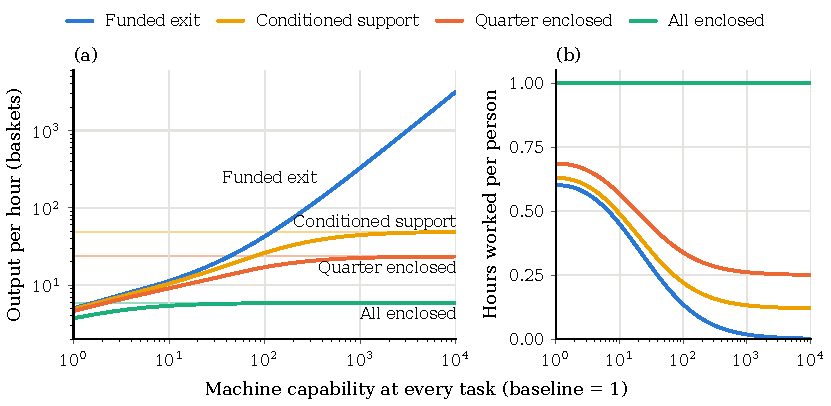
\includegraphics[width=0.88\textwidth]{figures/fig_paths.pdf}
\caption{Output per hour (a) and hours worked per person (b) along a path of machine progress in the instance of Section~\ref{sec:3.3}, under four rules for who can leave work: funded, unconditional exit for everyone ($\theta=\Delta=0$); support for everyone plus 0.3 baskets for working ($\Delta=0.3$); a quarter of people with no support outside work ($\theta=0.25$); and nobody with support ($\theta=1$). Machine capability is $1/\eta$, with relative human productivity $\eta\gamma(x)$ at every task. The thin horizontal lines are the ceilings $T/(hN_\infty)$ of Proposition~\ref{prop:2}. Drawn by code written with Claude (Anthropic).}
\label{fig:1}
\end{figure}

\subsection{The required return}\label{sec:4.3}

\begin{proposition}[the required return]\label{prop:3}
(i) At a given threshold $x$,
\[
\frac{\partial\log(w/r)}{\partial\log(\rho+\delta)}=\frac{1}{D(x)}\ge1,
\]
strictly if $a+\lambda\gamma(x)>0$, where $D(x)$ is land's share of a machine's build cost; and $w/P_s$ increases with $\rho$.
(ii) Whoever can leave work, the equilibrium with the lower required return has lower $w/r$, $w/P_s$ and labor's share, and a higher price of land in hours of work, $(r/\rho)/w$.
(iii) If $\theta=1$, the equilibrium threshold does not depend on $\rho$: a lower required return leaves hours, output and output per hour unchanged, and the elasticity of the price of land in hours of work with respect to $\rho$ is $-1-\rho/[(\rho+\delta)D(x^*)]$.
(iv) If $\theta<1$, a lower required return lowers labor supply at every threshold, strictly where $F$ has a positive density at $\log(1+\omega+\Delta)$: the threshold rises, hours fall, and output per hour rises.
\end{proposition}

Cheaper capital makes machine services cheaper relative to land, and since the wage at the threshold equals the cost of the machine services that replace an hour, the wage falls relative to rent. The chain amplifies the effect: machines are built with machine services, so a lower return cheapens them again at every round, and at a given threshold the elasticity is the inverse of the share of land, the one cost the return does not touch. Where people can leave work, the threshold rises as they do, which offsets part of the fall but never all of it: the wage in baskets falls, and with it the wage relative to rent (Appendix~\ref{app:A}). The price of land in hours of work rises twice, once because the rent is capitalized at a lower rate and once because the wage falls relative to the rent. Whether cheaper capital shows up as productivity depends on who can leave work. With nobody supported, only prices move. With funded exit, people leave work as the wage falls, and output per hour rises.

In the instance, land is 35 percent of a machine's build cost at the threshold with funded exit, so the elasticity in (i) is 2.87 there; at the threshold with nobody supported it is 1.96. A fall in the required return from 0.09 to 0.04 lowers $w/r$ by 52 percent and $w/P_s$ by 11 percent when nobody is supported, lowers labor's share from 0.58 to 0.51, and multiplies the price of land in hours of work by 4.7. With funded exit the same fall lowers $w/r$ by 60 percent and labor's share from 0.55 to 0.50; participation falls to 0.58, and output per hour rises 3 percent (Figure~\ref{fig:2}). These magnitudes depend on land's share of machine cost, which the instance was not set to match, and on the return required on productive capital, which fell much less than safe interest rates (Gomme, Ravikumar, and Rupert 2011; Caballero, Farhi, and Gourinchas 2017). They illustrate the proposition; they are not an estimate.

\begin{figure}[t]
\centering
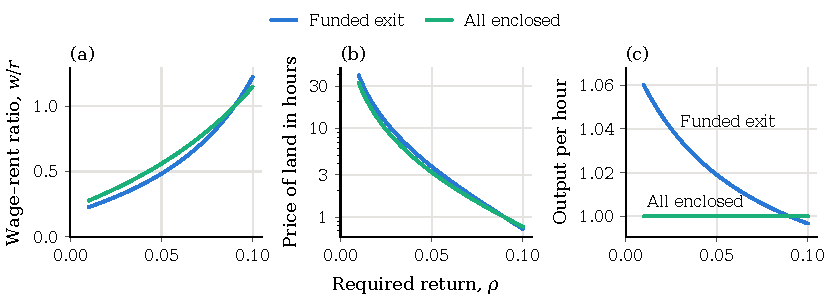
\includegraphics[width=0.88\textwidth]{figures/fig_rates.pdf}
\caption{The required return in the instance of Section~\ref{sec:3.3}, with funded exit for everyone and with nobody supported: (a) the wage--rent ratio, (b) the price of land in hours of work, $(r/\rho)/w$, and (c) output per hour, each relative to its value at $\rho=0.09$, for required returns from 0.04 to 0.10. Drawn by code written with Claude (Anthropic).}
\label{fig:2}
\end{figure}

\subsection{Prices}\label{sec:4.4}

\begin{lemma}[the price wedge]\label{lem:2}
Let consumption and measured output be bundles whose prices resolve into hours and land as $P_j=w\tilde L_j+r\tilde B_j$, where $\tilde L_j$ and $\tilde B_j$ count the hours and land along the bundle's chain of production with machines charged at their user cost. Then
\[
\frac{\partial\log(P_C/P_Y)}{\partial\log(r/w)}=\beta_C-\beta_Y,\qquad\beta_j=\frac{r\tilde B_j}{P_j},
\]
and for measured output of nominal value $P_YY$ produced with $N_a$ hours,
\begin{equation}\label{eq:13}
\frac{w/P_C}{Y/N_a}=\frac{wN_a}{P_YY}\cdot\frac{P_Y}{P_C}.
\end{equation}
\end{lemma}

With $\rho>0$ the requirements in Lemma~\ref{lem:2} are not the stationary requirements of \eqref{eq:4}: each round of machine-building is charged at $\rho+\delta$ rather than replaced at $\delta$, so interest is folded into hours and land. Whether consumption is more land-intensive than output is a question about these price requirements.

Real pay per hour, deflated by consumer prices, can fall behind output per hour, deflated by producer prices, for two reasons: labor's share falls, or consumer prices rise relative to producer prices. Lemma~\ref{lem:2} ties the second to the wage--rent ratio: when the wage falls relative to rent, consumer prices rise relative to producer prices if consumption is more land-intensive than measured output, as it is when consumption is heavy in shelter and output heavy in machines. Propositions~\ref{prop:2} and~\ref{prop:3} lower both labor's share and the wage--rent ratio, so they open both parts of the gap; absorption lowers the wage--rent ratio but, as Section~\ref{sec:4.1} showed, can raise labor's share. Section~\ref{sec:5} measures the split of the gap between the two.

\begin{lemma}[composition]\label{lem:3}
Let consumption be $C=\bigl[\alpha^{1/\sigma}c_M^{(\sigma-1)/\sigma}+(1-\alpha)^{1/\sigma}c_S^{(\sigma-1)/\sigma}\bigr]^{\sigma/(\sigma-1)}$ over a machine-made good $c_M$ and a bound good $c_S$, with $\alpha\in(0,1)$ and $\sigma>0$ ($\sigma=1$ read as the Cobb--Douglas limit), chosen at prices $p_M$, $p_S$.
(a) If $\sigma<1$ and $q=p_M/p_S\to0$ with $\dot q/q$ bounded, the bound good's share of spending tends to one, and measured consumption growth, the Divisia index $g_C=\dot c_S/c_S+s_M\sigma(-\dot q/q)$ with $s_M$ the machine-made good's share, tends to the growth of the bound good. For every $c_M$, $C<(1-\alpha)^{1/(\sigma-1)}c_S$.
(b) If $\sigma\ge1$, $C$ grows without bound as $c_M$ does, at any fixed $c_S$.
\end{lemma}

The bound good is any good whose supply machine progress cannot raise: space, which needs land, or care, which needs people. With an elasticity below one, the cheaper machine-made goods become, the smaller their share of spending, and measured growth converges to that of the bound goods (Baumol 1967; Ngai and Pissarides 2007). The level of consumption is then capped by the bound good, as it is by space in the basket of Section~\ref{sec:3}; with an elasticity of one or more it is not. The real-wage fork of B\r{a}ge and Wilson (2026) measures $q$ for durable goods against shelter: between 1964 and 2024 the consumer price of durable goods fell by a factor of 4.8 relative to that of shelter.

\subsection{The facts and what moves them}\label{sec:4.5}

Table~\ref{tab:facts} maps the facts of Section~\ref{sec:1} onto the results. No single primitive produces them all. Machine progress with hours that cannot fall produces slow growth of output per hour; machine progress and a lower required return each lower the wage relative to rent and labor's share whoever can leave work; absorption lowers output per hour at given technology. Two of the facts are inputs here rather than results: the required return, and who can leave work.

\begin{table}[htbp]
\centering
\caption{The facts and what moves them in the model.}
\label{tab:facts}
\footnotesize
\renewcommand{\arraystretch}{1.15}
\begin{tabular}{@{}>{\raggedright\arraybackslash}p{0.27\textwidth}>{\raggedright\arraybackslash}p{0.40\textwidth}>{\raggedright\arraybackslash}p{0.25\textwidth}@{}}
\toprule
Fact & In the model & Under which rules \\
\midrule
Slow growth of output per hour while machines improve & Machine progress (Proposition~\ref{prop:2}): output per hour converges to $T/(hN_\infty)$ and its elasticity with respect to capability to zero & When some hours cannot fall, $N_\infty>0$ \\
\addlinespace
Lower output per hour at given technology & More hours that cannot leave work, a higher $\theta$ or $\Delta$ (Proposition~\ref{prop:1}) & Any \\
\addlinespace
A falling labor share & Machine progress (Proposition~\ref{prop:2}); a lower required return (Proposition~\ref{prop:3}); absorption only for some schedules (Section~\ref{sec:4.1}) & Any \\
\addlinespace
The wage falling relative to rent; land dearer in hours of work & Machine progress, a lower required return, absorption (Propositions~\ref{prop:1}--\ref{prop:3}) & Any \\
\addlinespace
Consumer prices rising relative to producer prices & The wage falling relative to rent (Lemma~\ref{lem:2}) & Consumption more land-intensive than output \\
\addlinespace
Spending and hours moving to bound goods & Machine-made goods cheapening (Lemma~\ref{lem:3}) & An elasticity of substitution below one \\
\addlinespace
Low real interest rates & Not explained: the required return is a primitive & \\
\addlinespace
Hours per worker that stopped falling & Not explained: $\theta$ and $\Delta$ are primitives & \\
\bottomrule
\end{tabular}
\end{table}

\subsection{What the model leaves out}\label{sec:4.6}

\textbf{Welfare and policy.} The results describe measured output per hour, not welfare. A payment for working draws in people with work costs between $\log(1+\omega)$ and $\log(1+\omega+\Delta)$, who would not work for the wage alone; people without support work because they are poor, not because a price is wrong. Ranking such allocations needs a welfare criterion, which the paper does not supply. Nor does the model contain the instrument B\r{a}ge and Wilson (2026, Section~7) propose, a tax on the rent of land paid out as a uniform transfer: in the instance with funded exit, rent alone would pay for 0.38 of a basket per person, and support is paid mostly out of interest. Section~\ref{sec:7} returns to policy.

\textbf{Directed automation.} Technology is given here. If firms direct effort toward automating the tasks where automation saves most, cheap absorbed labor lowers the return to automating the tasks labor holds (Habakkuk 1962; Allen 2009; Acemoglu 2010). That would be a further channel from absorption to slower progress, which this paper does not model.

\textbf{Where $\theta$ comes from.} The share without support is a primitive here. When support is paid out of another household member's wage, it erodes as rents rise relative to wages, and $\theta$ becomes an outcome of the same prices; that version belongs to a study of the transition. Nor is the limit with people unsupported a living standard anyone could keep, since what their wage buys tends to zero: a floor under consumption would turn support, or departure from the market economy, from a primitive into an outcome.

\textbf{Dynamics.} The results compare stationary equilibria. They say where a path leads, not how fast it gets there: adjustment costs, the time it takes to build machines, and the timing of support are outside them.
% THEORY-NUMBERS-END

% DATA-NUMBERS-BEGIN
\section{Measurement}\label{sec:5}

This section measures the facts of Section~\ref{sec:1} and the implications of Section~\ref{sec:4}, in U.S. data from 1948 and in OECD data from 1995. Before any of the paper's data were pulled, apart from the series of output per hour that defines the eras, we wrote down what each measurement would compute, with a prediction and what would count against it for three of them and only what would count against it for a fourth, in a plan committed with its date to the paper's repository; the cross-country test of Section~\ref{sec:5.5} was fixed in every detail. Changes to the plan are logged with it, and Appendix~\ref{app:C} sets out the record. One change touched a measurement: the industry data of Section~\ref{sec:5.2} were not where the plan expected them, and the change of source was logged before any of its results were computed. Where a classification can be argued, we report the median over a grid of classifications with its range. Readings added after the data were seen are labeled exploratory. Every series was pulled on 16 November 2026 from its primary public source, and every number below is recomputed from the stored pull by checks that accompany the paper.

\subsection{The eras}\label{sec:5.1}

Figure~\ref{fig:3} shows output per hour in the nonfarm business sector with three series that moved with it. Output per hour grew 2.8 percent a year in 1948--73, 1.4 in 1973--95, 3.0 in 1995--2004, 1.5 in 2004--19 and 2.2 in 2019--25. Hours worked in the sector per person aged 16 and over fell 0.07 percent a year in 1948--73, rose 0.25 percent a year in 1973--95, and fell in every era since: 0.52 percent a year in 1995--2004, 0.22 in 2004--19 and 0.48 in 2019--25.\footnote{Annual averages of quarterly and monthly series (BLS, through FRED). The household survey was not collected in October 2025, during the shutdown of the federal government, so the population in 2025 is the average of eleven months. BLS introduces new population controls each January without revising earlier months, which puts steps into the series, the largest 1.1 percent in 2000 and 1.0 percent in 2025. With each January's change set to the average change of the other months of its year, a check added after the data were seen, hours per person grow 0.00, 0.30, $-0.35$, $-0.24$ and $-0.31$ percent a year over the five eras, and the ranking that follows is unchanged.} Since 1973 the four eras rank in exactly opposite orders by the two measures: the faster hours per person fell, the faster output per hour grew. The era 1948--73 breaks the ranking, with the fastest growth of output per hour and nearly flat hours per person. The ranking was not among the predictions written down before the data, and four eras are not a test: recessions in 2001 and 2020, the entry of women into paid work (Goldin 2006) and the retirement of a large generation all moved hours per person. The entry of women in particular, which carried hours per person up in 1973--95, raised productivity by putting talent where it was most productive (Hsieh, Hurst, Jones, and Klenow 2019), the opposite of absorption.

Lemma~\ref{lem:1} bounds what hours alone can do.\footnote{In the model, hours are total hours on a fixed endowment of land, so population growth alone would lower output per hour. The measurements divide hours by population or employment, which keeps that channel out.} At given technology, land and basket, the elasticity of output per hour with respect to hours lies between $-1$ and $0$, so the swing from hours per person falling 0.07 percent a year in 1948--73 to rising 0.25 in 1973--95 can account for at most 0.32 points a year of the slowdown of 1.3 points between the two eras, and for 0.19 at the instance's elasticity. Where the account explains more of the slowdown than that, it does so through composition (Lemma~\ref{lem:3}) and through what machine progress does when hours do not fall (Proposition~\ref{prop:2}), not through absorption at given technology.

On decade averages, labor's share of income in the sector fell 3.6 percent between 1948--57 and the 1990s and 9.3 percent between the 1990s and 2016--25; in 2025 it was at its lowest. The ten-year real interest rate estimated by the Federal Reserve Bank of Cleveland (Haubrich, Pennacchi, and Ritchken 2012) averaged 6.5 percent in 1982--84 and reached its low in 2020, $-0.12$ percent; the yield on ten-year inflation-indexed Treasury securities was $-0.60$ percent that year and 1.96 percent in 2025. Land's share of the market value of households' owner-occupied real estate, one minus the structures at current cost over the market value of the real estate, averaged 22 percent in 1952--72 and 37 percent in 2004--19; it peaked at 48 percent in 2005 and was 40 percent in 2025. Proposition~\ref{prop:3} reads these series together: a lower required return lowers the wage relative to rent and labor's share and raises the price of land in hours of work, whoever can leave work. The series moved in those directions. But the safe real rate is not the return required on productive capital, which fell much less (Section~\ref{sec:4.3}), and a lower discount rate raises the price of land on any account; the figure shows comovement, not the mechanism.

\begin{figure}[t]
\centering
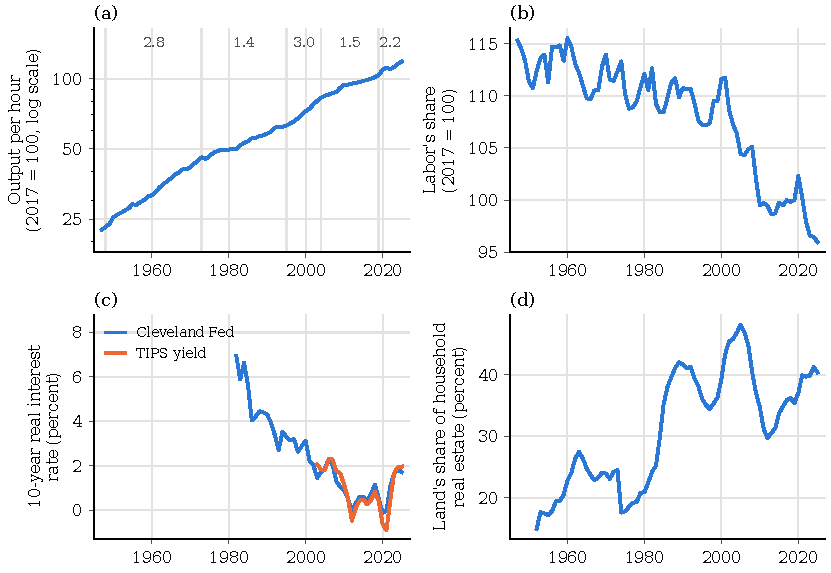
\includegraphics[width=0.88\textwidth]{figures/fig_eras.pdf}
\caption{U.S. series, annual averages. (a) Output per hour in the nonfarm business sector (index, 2017 = 100, log scale), with each era's growth in percent a year; (b) labor's share of income in the nonfarm business sector (index, 2017 = 100); (c) the ten-year real interest rate estimated by the Federal Reserve Bank of Cleveland, from 1982, and the yield on ten-year Treasury inflation-indexed securities, from 2003; (d) land's share of households' owner-occupied real estate, one minus residential structures at current cost over the real estate's market value, from 1952; as a residual it fell in 1974, when the market value of real estate fell while the current cost of structures rose. BLS, the Federal Reserve Bank of Cleveland, the Federal Reserve Board and the U.S. Treasury, through FRED, pulled 16 November 2026. Drawn by code written with Claude (Anthropic).}
\label{fig:3}
\end{figure}

\subsection{Where the slowdown lives}\label{sec:5.2}

The sector data are the BEA--BLS integrated industry-level production account, published by BEA: for 1947--2016, nominal gross output and intermediate inputs, their quantity indexes, and the hours of all workers, employees and self-employed, for 63 industries (44 before 1963; Eldridge et al. 2020); for 1997--2024, nominal value added, its quantity index and an index of hours (Garner, Harper, Russell, and Samuels 2026).\footnote{The plan named BEA's history of GDP by industry and the NIPA tables of hours by industry. BEA no longer publishes the first, for the years before 1997, on the industry classification used since; the production account that replaced both also counts the hours of the self-employed, which the NIPA tables leave out. The change of source was logged before any result was computed.} We aggregate the industries to 20 sectors, compute real value added by Törnqvist double deflation to 1997 and from the value-added indexes after, and carry hours forward from 1997 by the newer index.

Growth of output per hour in the sectors in scope splits each year into growth within sectors and the reallocation of hours,
\begin{equation}\label{eq:14}
g_{Y/H}=\sum_i\bar s_i\,(g_{Y_i}-g_{H_i})+\sum_i(\bar s_i-\bar h_i)\,g_{H_i},
\end{equation}
where $\bar s_i$ and $\bar h_i$ are sector $i$'s shares of value added and of hours, averaged over the two years. The second sum is negative when hours grow fastest where value added per hour is below average. The change in an era's growth against 1948--73 then splits exactly, with midpoint weights, into the slowdown within sectors, the shift of value added among sectors (Baumol's effect: shares moving toward sectors whose output per hour grows slowly), and the change in the reallocation of hours. We call the last two composition. The plan classed sectors by what binds them: machine-contestable (manufacturing, wholesale and retail trade, transportation and warehousing, information, finance and insurance, professional and technical services, management of companies, administrative services); site- and resource-bound (agriculture, mining, utilities, construction); and human-required, in person (education, health care and social assistance, arts and recreation, accommodation and food, other services). Real estate, whose owner-occupied output has no hours, and government are outside the baseline. Five other members of the grid move retail and administrative services to the human-required class, utilities to the machine-contestable class, government into the human-required class, real estate into the site-bound class, or accommodation and food into the site-bound class. The prediction was that composition is negative in 1973--95 and 2004--19 and accounts for at least a quarter of each era's slowdown in the median member of the grid; a tenth or less, or a positive sign, would count against.

Figure~\ref{fig:4} shows the split in the baseline. Output per hour in the sectors in scope grew 3.17 percent a year in 1948--73, 1.55 in 1973--95, 3.03 in 1995--2004, 1.33 in 2004--19 and 1.88 in 2019--24.\footnote{The scope is not the nonfarm business sector of Section~\ref{sec:5.1}: it includes agriculture, excludes real estate, and measures output as value added by industry.} The slowdown of 1.63 points a year in 1973--95 splits into 0.86 within sectors, 0.23 from the shift of value added and 0.54 from the reallocation of hours; the slowdown of 1.84 points in 2004--19 into 1.15, 0.23 and 0.46. The shift of value added toward slow sectors, Baumol's effect, is thus 14 and 13 percent of the two slowdowns; most of composition is the reallocation of hours. Over the grid, composition is 47 percent of the 1973--95 slowdown (the median; the range is 41 to 58) and 38 percent of the 2004--19 slowdown (38 to 47), and it is negative in every member. The members that only move a sector from one class to another leave the scope, and with it composition's total, unchanged: the median is the baseline's, and the other values come from the two members that add government or real estate to the scope. By the criterion written beforehand, the measurement supports the account. BEA's two files differ, though: over their overlap, 1998--2016, the newer gives growth of output per hour in the baseline scope of 1.93 percent a year and the older 1.59. On the older file alone, a check added after the data were seen, composition is 34 percent of the 2004--16 slowdown (the median over the grid; the range is 34 to 42), against 38 percent (38 to 47) on the spliced panel over the same years.

Much of the composition term, though, is the end of the farm exodus. Agriculture held 22 percent of the hours in scope in 1948 and 7 percent in 1973. As hours left a sector whose value added per hour was well below average, the reallocation term added 0.34 points a year to growth in 1948--73, a gain that could not recur. Agriculture alone accounts for 0.28 of the 0.54 points by which the reallocation term fell in 1973--95, and for 0.36 of the 0.46 points in 2004--19.\footnote{Each sector's piece of the reallocation term is $\bar s_i-\bar h_i$ times the growth of its hours less the growth of total hours. That reassigns the term among sectors without changing its total; without the subtraction, agriculture's pieces are 0.27 and 0.33.} Without agriculture, a reading added after the data were seen and not part of the verdict, composition is 27 percent of the 1973--95 slowdown and 19 percent of the 2004--19 slowdown: above a quarter in the first era and below it in the second, so partial by the same thresholds.

The larger part of each slowdown is within sectors: 53 percent in 1973--95 and 62 percent in 2004--19 in the baseline, with manufacturing the largest single piece in both. Construction, a site-bound sector, went from growth of output per hour of 2.3 percent a year in 1948--73 to declines of 0.5 percent a year in 1973--95 and 0.9 percent a year in 2004--19 (Goolsbee and Syverson 2023). The boom of 1995--2004 came despite composition: growth within sectors added 1.07 points a year more than in 1948--73, all of it in the machine-contestable sectors, while composition took away 1.21 points, more than in either slow era. Composition thus lowers growth in every era since 1973 against 1948--73, and most in the boom; what separates the slow eras from the fast one is growth within sectors. And hours moved toward work done in person: the human-required sectors' share of hours rose from 14 percent in 1948 to 34 percent in 2024, and their share of value added from 10 to 20 percent.

Composition is a necessary implication of the account, not a test of its mechanism. Lemma~\ref{lem:3} and absorption predict it, and so does any account of structural change (Baumol 1967; Ngai and Pissarides 2007). The classification does not separate goods bound by land or by people from goods whose productivity grows slowly for other reasons.

\begin{figure}[t]
\centering
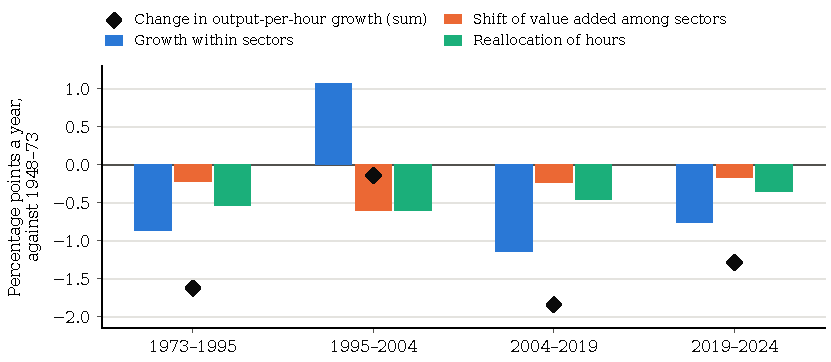
\includegraphics[width=0.88\textwidth]{figures/fig_industry.pdf}
\caption{The change in the growth of output per hour against 1948--73, in percentage points a year, split by \eqref{eq:14} into the slowdown within sectors, the shift of value added among sectors, and the change in the reallocation of hours; the diamonds mark the sum. The baseline member of the grid: U.S. private sectors other than real estate. BEA--BLS integrated industry-level production account (Eldridge et al. 2020; Garner, Harper, Russell, and Samuels 2026), hours of all workers. Drawn by code written with Claude (Anthropic).}
\label{fig:4}
\end{figure}

\subsection{Pay against productivity}\label{sec:5.3}

Between 1973 and 2024, output per hour in the nonfarm business sector rose 92 log points and hourly compensation deflated by the consumer price index (CPI) rose 40, a gap of 52 points (Figure~\ref{fig:5}). By \eqref{eq:13} the gap splits exactly into the fall in labor's share, 14 points, and the rise of consumer prices relative to the sector's output prices, 38 points, or 73 percent of the gap.\footnote{Labor's share here is compensation over the sector's current-dollar output, as implied by the series compared. The share BLS publishes falls 15 log points over the same years.} That a large part of the gap is a gap between prices is known (Feldstein 2008; Stansbury and Summers 2017). Lemma~\ref{lem:2} says what the price wedge measures: when the wage falls relative to rent, consumer prices rise relative to producer prices if consumption is more land-intensive than output. The prediction was that the wedge rises and that removing shelter from consumer prices removes at least a third of the rise, with less than a tenth counting against. Measured against the CPI less shelter the wedge is 24 points, so shelter accounts for 37 percent of it. From 1983, when the CPI began to price owner-occupied housing by rental equivalence, the gap is 42 points, the wedge 31, or 73 percent of the gap, and shelter's part 34 percent. The measurement supports the prediction, narrowly in the later window. For comparison, removing energy removes 4 percent of the wedge over 1973--2024 and widens it by 6 percent from 1983; removing medical care, a service that requires people, removes 13 percent in both windows.

The test is close to mechanical, though. Owner-occupied housing is outside the nonfarm business sector and weighs heavily in the CPI, so any rise in the relative price of shelter opens the wedge, whatever raised it: land, the cost of building, limits on building, or how the CPI measures rents. The measurement shows where the wedge is, not that a falling wage relative to rent put it there. The wedge also holds the CPI's own biases and the prices of investment goods and imports. And the pay here is average pay: the gap for the typical worker is wider, by the rise in inequality (Stansbury and Summers 2017).

\begin{figure}[t]
\centering
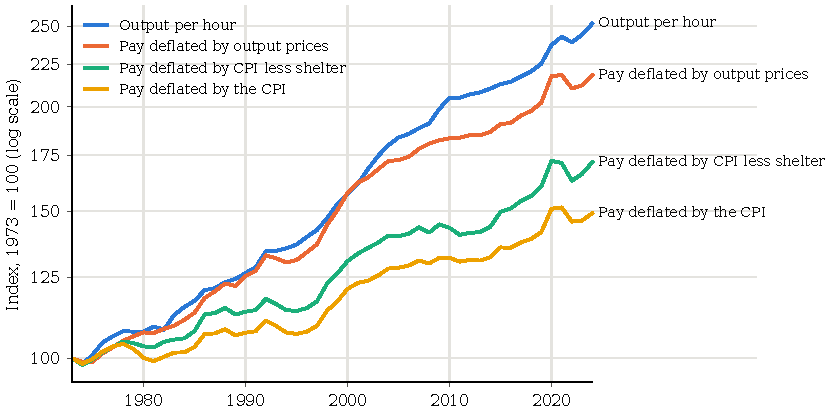
\includegraphics[width=0.88\textwidth]{figures/fig_gap.pdf}
\caption{Output per hour and hourly compensation in the U.S. nonfarm business sector, 1973 = 100 (log scale), with compensation deflated by the sector's output prices, by the CPI less shelter, and by the CPI. The distance between output per hour and compensation deflated by output prices is the fall in labor's share; between compensation deflated by output prices and by the CPI, the rise of consumer relative to producer prices; between compensation deflated by the CPI less shelter and by the CPI, shelter's part of that rise. BLS through FRED, annual averages, pulled 16 November 2026. Drawn by code written with Claude (Anthropic).}
\label{fig:5}
\end{figure}

\subsection{The hours that did not fall}\label{sec:5.4}

Average annual hours per person engaged in the United States fell from 2,022 in 1950 to 1,840 in 1980, or 0.31 percent a year, and then to 1,789 in 2023, or 0.07 percent a year (Penn World Table 11.0; Feenstra, Inklaar, and Timmer 2015). In Germany, France, the United Kingdom, the Netherlands and Sweden, taken together as a geometric mean, they fell 0.86 percent a year before 1980 and 0.27 percent a year after (Figure~\ref{fig:6}). Had U.S. hours per worker kept to their 1950--80 trend, they would have been 1,608 in 2023, 10.1 percent fewer than they were; had they followed the European path from their 1980 level, 1,636, or 8.6 percent fewer.

Lemma~\ref{lem:1} maps hours into output per hour at given technology, land and basket. At the instance's elasticity, $-0.59$, output per hour in 2023 would have been 6.5 percent higher on the U.S. trend, or 0.15 points a year over 1980--2023, and between 4.3 and 11.2 percent higher (0.10 to 0.25 points a year) for elasticities between $-0.4$ and $-1$; on the European path, 5.4 percent higher (3.6 to 9.4). Set against the slowdown, its size depends on the windows compared, so we state no share: the 0.15 points are 17 percent of the fall in the growth of output per hour from 2.76 percent a year in 1948--73 to 1.91 in 1980--2023, but 46 percent of the smaller fall from 2.22 in 1950--80, the window of the hours trend, and 7 percent when hours and output per hour are both broken at 1973.\footnote{The hours are the whole economy's (Penn World Table); output per hour is the nonfarm business sector's.} The mapping holds employment as it was and attributes nothing. It is an envelope for what the hours that stopped falling could have cost, and it does not say how many of them could not fall: that share is $\theta$, a primitive of the model, and the paper does not measure it. Since 1980 long hours have become more common among men with high pay and less common among men with low pay (Kuhn and Lozano 2008), continuing a reversal under way since the 1890s (Costa 2000): the hours that stopped falling are not mostly those of people the model has working for want of support. With machines that use less land than in the instance, on the other hand, the elasticity would be nearer $-1$ (Section~\ref{sec:4.1}) and the envelope nearer its upper end.

Europe is the obvious objection. Its hours per worker fell faster than America's before 1980 and after, and its support outside work is more generous, yet its output per hour grew more slowly than America's after 1995, with the gap in market services that use information technology (van Ark, O'Mahony, and Timmer 2008). The account reads part of Europe's higher level of output per hour around 1995 as the product of its fewer hours (Bourl\`es and Cette 2007), and notes that the fall in Europe's hours slowed after 1980 by more than America's did, by 0.59 points a year against 0.25. It does not explain why information technology spread more slowly in European services.

\begin{figure}[t]
\centering
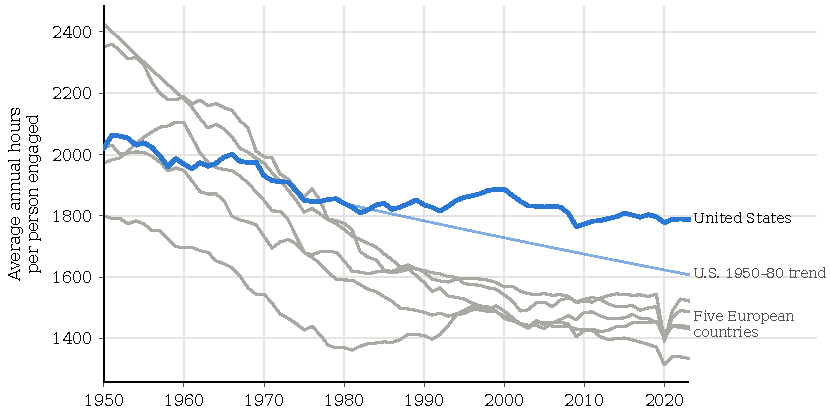
\includegraphics[width=0.88\textwidth]{figures/fig_hours.pdf}
\caption{Average annual hours worked per person engaged, 1950--2023: the United States, its 1950--80 trend extended, and Germany, France, the United Kingdom, the Netherlands and Sweden. Penn World Table 11.0. Drawn by code written with Claude (Anthropic).}
\label{fig:6}
\end{figure}

\subsection{Across countries: the frozen test}\label{sec:5.5}

Proposition~\ref{prop:1} says that where more hours are pushed into work, output per hour is lower. Across countries, then, faster growth of hours per working-age person should go with slower growth of output per hour, if absorption is what moves hours. We fixed the test in writing before pulling its data. The sample is the OECD members with complete annual data for 1995--2019, excluding Ireland, whose GDP moved with multinationals' accounting from 2015, and Luxembourg, many of whose workers live abroad; the end year avoids the pandemic. The primary regression is of the annualized log growth of GDP per hour worked at constant purchasing power parities (OECD Productivity Database) on that of hours worked per person aged 15--64, with the 1995 level of GDP per hour as a control for catching up and heteroskedasticity-robust (HC1) standard errors (MacKinnon and White 1985). The secondary is the same relation over five-year periods with country and period effects, with inference by a wild cluster bootstrap with Webb weights and 9,999 draws (Cameron, Gelbach, and Miller 2008; Webb 2023). The rule: consistent with the account if the coefficient is negative with a two-sided $p<0.05$ in the primary and negative in the secondary; counts against it if the coefficient is positive with $p<0.05$ in the primary; uninformative otherwise.

The sample has 33 countries; Colombia, Estonia and Korea lack some years. Across countries the coefficient is $+0.33$ (standard error 0.38, $p=0.39$; Figure~\ref{fig:7}a): positive, the opposite of the prediction, and far from significant. Within countries it is $-0.25$, with a bootstrap $p$-value of 0.013 (Figure~\ref{fig:7}b). By the rule fixed beforehand the test is uninformative. The robustness checks declared with it do not change the reading. Dropping one country at a time leaves the cross-country coefficient between 0.06 and 0.46, never significant. Since hours sit in both variables, errors in measuring them bias the coefficient down (Borjas 1980); instrumenting the OECD measure of hours by the Penn World Table's gives $+0.16$ ($p=0.72$), though the two measures may share sources, which would make the correction partial.

The two estimates answer different questions. The cross-country coefficient compares long-run paths, along which technology and demand raise hours and output per hour together while absorption moves them apart. A negative coefficient is what the account implies if absorption dominates; the estimate neither shows that it does nor, with a standard error of 0.38, rules it out. The within-country coefficient compares five-year spells, which also contain the cycle: when a recession sheds low-paid hours first, hours fall and measured output per hour rises, with no absorption in it, and in the United States output per hour has moved against hours over the cycle since the mid-1980s (Gal\'i and van Rens 2021). And the within estimate is the one most exposed to errors in hours, against which the instrument was declared only for the primary. Its sign is the account's, and its size is less than half of Lemma~\ref{lem:1}'s elasticity in the instance; neither was the test.

\begin{figure}[t]
\centering
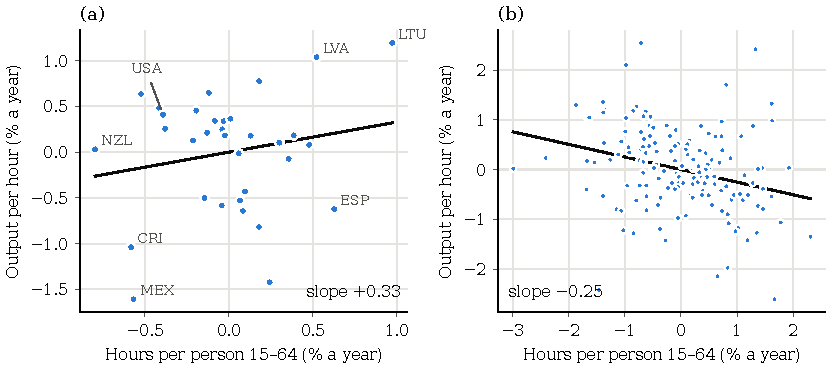
\includegraphics[width=0.88\textwidth]{figures/fig_hx.pdf}
\caption{Growth of GDP per hour worked against growth of hours worked per person aged 15--64, 33 OECD countries, annualized log growth in percent a year. (a) Across countries, 1995--2019, each variable net of the 1995 level of GDP per hour (an added-variable plot; slope $+0.33$). (b) Within countries, five periods from 1995 to 2019, each variable net of country and period effects (slope $-0.25$). OECD Productivity Database and population by age, pulled 16 November 2026. Drawn by code written with Claude (Anthropic).}
\label{fig:7}
\end{figure}

\subsection{Since 2019}\label{sec:5.6}

Output per hour grew 2.25 percent a year between 2019 and 2025, against 1.50 in 2004--19, and 2.20 percent a year from the fourth quarter of 2019 to the third quarter of 2026. Hours per person aged 16 and over fell 0.48 percent a year, against 0.22 in 2004--19, or 0.31 against 0.24 with the January steps in the population smoothed (Section~\ref{sec:5.1}). The average hourly earnings of production and nonsupervisory employees, most of private employment, rose from 0.840 to 0.860 of those of all private employees, or 0.40 percent a year, against 0.07 percent a year in 2007--19; the plan used this ratio as its index of compression. The plan stated no prediction for these years, since the pickup in output per hour was known when it was written; it said only that faster output per hour with rising hours per person and no compression would count against the account. What happened is the opposite combination, the one Proposition~\ref{prop:1} gives when hours leave work. Other accounts predict it too. The population aged 16 and over aged as a large generation retired, which in the model's terms is funded exit for the old, and the compression came in a tight labor market (Autor, Dube, and McGrew 2023).

\section{Predictions and what would count against them}\label{sec:6}

Table~\ref{tab:pred} lists the three predictions and the one further condition as they were written before the data were pulled, what would have counted against each, and what Section~\ref{sec:5} found. Two predictions support the account, one narrowly, and the composition result is partial once the end of the farm exodus is set aside. The frozen cross-country test is uninformative. Nothing counted against the account after 2019; what happened is what it gives when hours leave work, and what other accounts predict too.

\begin{table}[t]
\centering
\caption{What the plan said before the data were pulled, and what the data said.}
\label{tab:pred}
\footnotesize
\renewcommand{\arraystretch}{1.15}
\begin{tabular}{@{}>{\raggedright\arraybackslash}p{0.28\textwidth}>{\raggedright\arraybackslash}p{0.16\textwidth}>{\raggedright\arraybackslash}p{0.33\textwidth}>{\raggedright\arraybackslash}p{0.14\textwidth}@{}}
\toprule
Prediction & Would count against & Measured & Reading \\
\midrule
Composition, the shift of value added toward slow sectors and the reallocation of hours, is negative and at least a quarter of the slowdowns of 1973--95 and 2004--19 against 1948--73 (Section~\ref{sec:5.2}) & A tenth or less, or a positive sign & 47 and 38 percent (medians over the grid; ranges 41--58 and 38--47). Without agriculture, exploratory: 27 and 19 percent & Supports; partial without agriculture \\
\addlinespace
Consumer prices rise relative to producer prices, and removing shelter removes at least a third of the rise (Section~\ref{sec:5.3}) & Less than a tenth & A wedge of 38 log points over 1973--2024 and 31 over 1983--2024; shelter is 37 and 34 percent of it & Supports, narrowly \\
\addlinespace
Across OECD countries, 1995--2019, faster growth of hours per person aged 15--64 goes with slower growth of output per hour (Section~\ref{sec:5.5}) & A positive coefficient with $p<0.05$ & Across countries $+0.33$ ($p=0.39$); within countries $-0.25$ (bootstrap $p=0.013$) & Uninformative \\
\addlinespace
After 2019: none stated, since the pickup in output per hour was known; only what would count against the account (Section~\ref{sec:5.6}) & Faster output per hour with rising hours per person and no compression & Output per hour 2.25 percent a year against 1.50; hours per person falling 0.48 percent a year; compression 0.40 percent a year & Does not count against \\
\bottomrule
\end{tabular}
\end{table}

The measurements also bear on the rivals of Section~\ref{sec:2}, though the plan contained no test that separates the account from any of them.

\textbf{Exhausted opportunities.} Most of each slowdown is within sectors, and so is what separates the slow eras from the boom of 1995--2004; that is where a slower frontier would show (Bloom, Jones, Van Reenen, and Webb 2020). Growth accounting puts much of each slowdown in total factor productivity (Fernald 2015), while absorption at given technology works through capital per hour. On this account the part in total factor productivity would come from Proposition~\ref{prop:2}, machine progress that does not raise output per hour, which these data cannot tell from a slower frontier. The account does not need the frontier to slow, and nothing here shows that it did not.

\textbf{Structural change.} Composition lowers growth in every era since 1973, and most in the boom of 1995--2004, so it accounts for part of the gap with 1948--73 but not for the timing of the slow eras. Lemma~\ref{lem:3} is Baumol's mechanism with the bound goods named, and the measurement cannot tell bound goods from goods whose productivity grows slowly for other reasons.

\textbf{Energy.} Energy prices do not account for the rise of consumer relative to producer prices: removing energy from the CPI barely changes it, while removing shelter removes a third of it. That says nothing against the energy account of the slowdown in industries' productivity growth (Jorgenson 1988), which works through costs rather than through the gap between consumer and producer prices.

\textbf{Demand and the interest rate.} Low real rates came with a lower labor share and with land accounting for more of the value of housing, as Proposition~\ref{prop:3} says they would through the supply side. A demand account in which rates fall for other reasons predicts the rise in land's share as well, through capitalization, and the plan had no test to separate the two.

\textbf{Labor-market reforms.} The cross-country test re-measured the trade-off between employment and productivity that Dew-Becker and Gordon (2012) found in Europe after the reforms of the late 1990s. Across countries over 1995--2019 it does not appear. Within countries over five-year spells a negative association does, though the cycle and errors in measured hours could produce it without absorption (Section~\ref{sec:5.5}).

\textbf{Mismeasurement and market power.} Nothing here tests either.

\section{Conclusion}\label{sec:7}

Output per hour is the inverse of the hours an economy uses per unit of output. In a task economy whose prices resolve into hours and the rents of what cannot be produced, and whose consumption needs land, machine progress raises output toward a limit set by land, and output per hour beyond that only as hours are released. When some hours cannot leave work, output per hour converges to a ceiling, land per remaining hour over land per basket. Under every rule further progress lowers the wage relative to rent and moves income to the owners of land, and a lower required return does the same to prices. One cost system, moved by a few primitives, thus connects faces of the great stagnation that are usually studied apart: slow growth of measured productivity alongside fast machine progress, a falling labor share, real interest rates that fell for four decades, land that came to account for more of the value of housing, and a gap between pay and productivity that is mostly a gap between consumer and producer prices.

The measurements give the account less than its theory allows. By the criteria written beforehand, composition is a large part of each slowdown and shelter is a third of the price wedge. But much of the composition is the end of the farm exodus, and composition took even more from the boom of 1995--2004. Had hours per worker kept falling after 1980, output per hour would, at given technology, have grown 0.15 points a year faster at the instance's elasticity, and at most 0.25. The cross-country test of absorption is uninformative, and the test of the price wedge shows where the wedge is rather than what put it there. Most of each slowdown is within sectors, and so is what separates the slow eras from the boom; there a slower frontier and the ceiling of Proposition~\ref{prop:2} look alike in these data. And the ceiling itself rests on a basket in which nothing replaces land (Section~\ref{sec:4.2}). The sharpest test the account suggests is Proposition~\ref{prop:2}(iv): among economies that share a technological frontier, output per hour should respond less to machine capability where more hours cannot leave work. That test needs a measure of how many hours cannot leave, which this paper does not have.

\textbf{Policy.} The model ranks no allocations, since it has no welfare criterion. What it says is how the rules for who can leave work move measured output per hour and hours; in the limit they move neither output, which land caps, nor labor's share, which tends to zero under every rule. Support that does not depend on work lets hours fall as wages fall, and output per hour then keeps rising with machine capability; evidence on unconditional transfers finds that hours do fall, modestly (Cesarini, Lindqvist, Notowidigdo, and \"Ostling 2017; Vivalt et al.\ 2024). A payment for working leaves hours that do not fall even when the wage buys nothing, as a population without support does, and with them a ceiling (Proposition~\ref{prop:2}). Denser use of land lowers land per basket and raises the ceiling. A tax on the rent of land paid out as a uniform transfer, which B\r{a}ge and Wilson (2026, Section~7) propose, is not modeled here. Rent alone would pay for 0.38 of a basket per person in the instance with funded exit, of the same order as the coverage ratio they measure for the United States, 0.30 in 2025 (0.15 to 0.59 across their measures). On either count a rent dividend pays for part of a basket, and the rest of any support would come from interest or from taxes on other bases.

\textbf{Artificial intelligence.} Artificial intelligence improves machines at many tasks at once, though not uniformly as Proposition~\ref{prop:2}'s $\eta$ does. On this account its effect on measured productivity depends on whether hours are released as much as on what it can do. Under every rule it would lower the wage relative to rent and labor's share; what the rules decide is whether output per hour keeps rising, which past the ceiling it does only as hours fall. Growth can stay bounded by the tasks hardest to automate even as automation spreads (Aghion, Jones, and Jones 2019), a version of Lemma~\ref{lem:3}, and so far there is no sign of the acceleration that rapid automation would bring (Nordhaus 2021); measured productivity can also lag a new general-purpose technology while firms build the intangible capital it needs (Brynjolfsson, Rock, and Syverson 2021). The account's own prediction is comparative: among economies that adopt the same technology, measured gains in output per hour will be larger where hours per person fall, or where support outside work does not depend on working.
% DATA-NUMBERS-END

\appendix
\counterwithin{equation}{section}
\counterwithin{table}{section}
\titleformat{\section}{\normalfont\Large\bfseries}{Appendix~\thesection.}{0.6em}{}

% THEORY-NUMBERS-BEGIN
\section{Proofs}\label{app:A}

Write $v=w/r$ and set $r=1$.

\textbf{The labor market: one clearing threshold.} On $(0,x_c)$,
\[
L_s'(x)=-1+\frac{\lambda\delta\gamma(x)}{1-a\delta},\qquad
1-a\delta-\lambda\delta\gamma(x)=D(x)+\rho\bigl(a+\lambda\gamma(x)\bigr)>0,
\]
so $L_s'<0$, and $B_s'(x)=b\delta\gamma(x)/(1-a\delta)>0$. Labor demand $n_D=TL_s/B_s$ is therefore strictly decreasing. The wage $v=\gamma p_m$ rises strictly with $x$, since $\gamma$ is strictly increasing and $p_m=(\rho+\delta)b/D(x)$ is nondecreasing ($D$ falls as $\gamma$ rises, with $\lambda\ge0$). Since $v=\gamma p_m$, the wage in baskets satisfies
\begin{equation}\label{eq:A1}
\frac{1}{\omega}=\frac{P_s}{v}=m(x)+\frac{h}{v(x)},\qquad m(x)=1-x+\frac{J(x)}{\gamma(x)},
\end{equation}
and $m$ is nonincreasing: for $x<y$, $J(y)\le J(x)+(y-x)\gamma(y)$ and $\gamma(x)\le\gamma(y)$ give $J(y)/\gamma(y)\le J(x)/\gamma(x)+(y-x)$, so $m(y)\le m(x)$. Hence $\omega$ rises strictly with $x$, and $n_S$ is nondecreasing. If $x_c<1$, $v$ and $P_s$ grow without bound as $x$ approaches $x_c$, but $\omega$ does not: it equals $(\rho+\delta)b\gamma/[(\rho+\delta)b(\gamma(1-x)+J)+hD]$, finite at $D=0$. Since $n_D(0)=T/h>N\ge n_S(0)$ and $n_S(x_c)>n_D(x_c)$ by assumption, exactly one threshold in $(0,x_c)$ clears the labor market. Substituting \eqref{eq:2}--\eqref{eq:4} gives $P_sY=vN_a+T+\rho V_mX$. If support is funded, \eqref{eq:7}, the provider consumes $(T+\rho V_mX)/P_s-(1-\theta)N-\Delta N_a\ge0$ baskets, baskets consumed sum to $Y$, and the threshold is an equilibrium.

\begin{proof}[Proof of Lemma~\ref{lem:1}]
$Y/N_a=(T/B_s)/(TL_s/B_s)=1/L_s$, and the signs were shown above. Along a change that moves $x^*$ with technology, $T$ and $h$ fixed, $d\log\pi=-(L_s'/L_s)\,dx^*$ and $d\log N_a=(L_s'/L_s-B_s'/B_s)\,dx^*$. Dividing gives \eqref{eq:9}, which lies in $(-1,0)$ since $\psi>0$.
\end{proof}

\begin{proof}[Proof of Proposition~\ref{prop:1}]
Technology fixes $n_D$. The excess demand $n_D-n_S^1$ is strictly decreasing and negative at $x^*_0$, where $n_D(x^*_0)=n_S^0(x^*_0)<n_S^1(x^*_0)$, so its zero $x^*_1$ lies below $x^*_0$. Then $N_a=n_D$ is higher, $Y=T/B_s$ is higher, $\pi=1/L_s$ is lower, and $v$ and $\omega$, both increasing in $x$, are lower. For the parameters, $\partial n_S/\partial\theta=N[1-F(\cdot)]$, positive where some people with support do not work, and, where $F$ has a density $f$, $\partial n_S/\partial\Delta=N(1-\theta)f(\cdot)/(1+\omega+\Delta)$, positive where $f>0$.
\end{proof}

\begin{proof}[Proof of Proposition~\ref{prop:2}]
Write $\gamma_\eta=\eta\hat\gamma$ and $J_\eta=\eta\hat J$. For small $\eta$, $D_\eta(1)=1-(\rho+\delta)(a+\lambda\eta\hat\gamma(1))\ge\underline D=[1-(\rho+\delta)a]/2>0$, so $x_c=1$ and $D_\eta\ge\underline D$ on $[0,1]$.

(i) $v=\eta\hat\gamma(x)(\rho+\delta)b/D_\eta(x)\le\eta\hat\gamma(1)(\rho+\delta)b/\underline D\to0$ uniformly in $x$, and $\omega\le v/h$ since $P_s\ge h$. Labor's share is $vN_a/(P_sY)=\omega N_a/Y\le\omega N/Y$, with $Y\ge T/[h+b\delta\hat J(1)/(1-a\delta)]$ for $\eta\le1$; it tends to zero.

(ii) $N_a=n_S(x^*)$ tends to $N_\infty$ by continuity of $F$, since $\omega(x^*)\to0$.

(iii) $h\le B_s(x^*)\le h+\eta b\delta\hat J(1)/(1-a\delta)$, so $Y\to T/h$, and $\pi=Y/N_a$ gives the limits.

\emph{Interiority.} For small $\eta$, $x_c=1$ and $n_D(0)=T/h>N\ge n_S(0)$, so a clearing threshold in $(0,1)$ exists if $n_S(1)>n_D(1)$. If $N_\infty>0$, $n_S(1)\ge N\theta+N(1-\theta)F(\log(1+\Delta))=N_\infty$ while $n_D(1)=T\lambda\delta\eta\hat J(1)/[(1-a\delta)B_s(1)]\to0$. If $\lambda=0$, $n_D(1)=0$, and $n_S(1)>0$ when $F(z)>0$ for every $z>0$, since $\omega(1)>0$. The case of \eqref{eq:12} is treated in (iv). \emph{Funding.} As $\eta\to0$, $P_s\to h$, $N_a\to N_\infty$, and interest $\rho V_mX\to0$, since $V_m=b/D_\eta$ is bounded and $X=Y\eta\hat J(x^*)/(1-a\delta)\to0$; so \eqref{eq:7} holds for small $\eta$ when $T>h[(1-\theta)N+\Delta N_\infty]$.

(iv) Extend $\hat\gamma$ to a continuously differentiable function on a neighborhood of $[0,1]$, and $F$ linearly below zero (which changes nothing, since $\omega\ge0$). Let $G(x,\eta)=TL_s(x;\eta)/B_s(x;\eta)-n_S(x;\eta)$. Near $\eta=0$, $G$ is continuously differentiable: $L_s$ and $B_s$ are linear in $\eta$, and $\omega=\eta(\rho+\delta)b\hat\gamma/[\eta(\rho+\delta)b(\hat\gamma(1-x)+\hat J)+hD_\eta]$ is smooth with a denominator near $hD_0>0$. At $\eta=0$, $G(x,0)=T(1-x)/h-N_\infty$ and $\partial G/\partial x=-T/h\neq0$. For each $\eta$, $G(\cdot,\eta)$ is strictly decreasing on $(0,x_c)$, so the branch the implicit function theorem gives is the unique clearing threshold.

If $N_\infty>0$, $G(\cdot,0)$ vanishes at $x_0=1-hN_\infty/T\in(0,1)$, since $0<hN_\infty\le hN<T$. By the implicit function theorem $x^*(\eta)$ is continuously differentiable near zero with $x^*(0)=x_0$, and $\pi(\eta)=1/L_s(x^*(\eta);\eta)$ is continuously differentiable with $\pi(0)=T/(hN_\infty)>0$. Then $d\log\pi/d\log(1/\eta)=-\eta\pi'(\eta)/\pi(\eta)\to0$.

If $N_\infty=0$, then $\theta=\Delta=0$, and $G(1,0)=0$, so $x^*(\eta)$ is continuously differentiable near zero with $x^*(0)=1$. Along it, $N_a(\eta)=NF\bigl(\log(1+\omega(x^*(\eta);\eta))\bigr)$, where $\omega(x;0)=0$ and $\partial\omega/\partial\eta(1,0)=\hat\kappa=(\rho+\delta)b\hat\gamma(1)/[h(1-(\rho+\delta)a)]>0$, so $N_a'(0)=Nf(0)\hat\kappa>0$. On the demand side $N_a'(0)=(T/h)[-x^{*\prime}(0)+\lambda\delta\hat J(1)/(1-a\delta)]$; equating the two, $x^{*\prime}(0)<0$ exactly when \eqref{eq:12} holds, in which case $x^*(\eta)<1$ for small $\eta>0$ and the thresholds are interior. Since $N_a(\eta)=N_a'(0)\eta+o(\eta)$ with $N_a'$ continuous, $d\log N_a/d\log\eta\to1$; $Y$ is continuously differentiable with $Y(0)=T/h$, so $d\log Y/d\log\eta\to0$. Hence $d\log\pi/d\log(1/\eta)\to1$.
\end{proof}

\begin{proof}[Proof of Proposition~\ref{prop:3}]
(i) With $c=\rho+\delta$ and $A=a+\lambda\gamma(x)$, $v=\gamma(x)cb/(1-cA)$, so $\partial\log v/\partial\log c=1+cA/(1-cA)=1/D(x)$, which exceeds one when $A>0$; and $V_m=p_m/c=b/D$, so $D=b/V_m$. Further, $\omega=\gamma/[\gamma(1-x)+J+h/p_m]$ with $p_m=cb/(1-cA)$ increasing in $c$, so $\omega$ increases with $\rho$.
(ii) Let the required return fall, so that $c$ falls from $c_0$ to $c_1$, and let $x_0$, $x_1$ be the equilibrium thresholds and $\omega_0$, $\omega_1$ the wages in baskets. By (i), $\omega(x;c)$ falls at every $x$, so $n_S(x;c)$ falls weakly at every $x$, while $n_D$ does not depend on $c$; hence $x_1\ge x_0$. If $x_1=x_0$, then $\omega_1=\omega(x_0;c_1)<\omega(x_0;c_0)=\omega_0$. If $x_1>x_0$, then $n_S(x_1;c_1)=n_D(x_1)<n_D(x_0)=n_S(x_0;c_0)$, and since $n_S$ depends on $c$ only through $\omega$ and is nondecreasing in it, again $\omega_1<\omega_0$. By \eqref{eq:A1}, $v=h/[1/\omega-m(x)]$ with $m$ nonincreasing, so $v_1<v_0$. Labor's share is $vN_a/(P_sY)=\omega L_s(x^*)$, lower since $\omega$ falls and $L_s$ is decreasing. A unit of land yields $r$ a period; at the required return it is worth $r/\rho$, or $1/(\rho v)$ hours of work, which rises as $\rho$ and $v$ fall.
(iii) With $\theta=1$, $n_S\equiv N$, and $n_D=TL_s/B_s$ does not involve $\rho$; nor, then, do $x^*$, $N_a$, $Y$ and $\pi$. The elasticity of $1/(\rho v)$ with respect to $\rho$ is $-1-\partial\log v/\partial\log\rho=-1-\rho/[(\rho+\delta)D]$, by (i) at the fixed threshold.
(iv) By (i), $\omega(x)$ rises with $\rho$ at every $x$, so $n_S(x)$ is nondecreasing in $\rho$, and increasing where $F$ has a positive density at $\log(1+\omega+\Delta)$. A lower $\rho$ therefore shifts supply down at every threshold, and the argument of Proposition~\ref{prop:1}, reversed, gives the result.
\end{proof}

\begin{proof}[Proof of Lemma~\ref{lem:2}]
$P_j/w=L_j+(r/w)B_j$, so
\[
\frac{\partial\log(P_C/P_Y)}{\partial\log(r/w)}=\frac{(r/w)B_C}{P_C/w}-\frac{(r/w)B_Y}{P_Y/w}=\beta_C-\beta_Y.
\]
Equation~\eqref{eq:13} multiplies and divides by $P_Y$.
\end{proof}

\begin{proof}[Proof of Lemma~\ref{lem:3}]
Demand gives $c_M/c_S=[\alpha/(1-\alpha)]q^{-\sigma}$, so $s_M=\alpha q^{1-\sigma}/[\alpha q^{1-\sigma}+1-\alpha]\to0$ as $q\to0$, since $1-\sigma>0$. The Divisia index grows at $s_M\dot c_M/c_M+(1-s_M)\dot c_S/c_S=\dot c_S/c_S+s_M\sigma(-\dot q/q)$, which tends to $\dot c_S/c_S$ when $s_M\to0$ and $\dot q/q$ is bounded. For the level, $(\sigma-1)/\sigma<0$, so $C^{(\sigma-1)/\sigma}>(1-\alpha)^{1/\sigma}c_S^{(\sigma-1)/\sigma}$; raising both sides to the negative power $\sigma/(\sigma-1)$ gives $C<(1-\alpha)^{1/(\sigma-1)}c_S$. (b) If $\sigma>1$, $(\sigma-1)/\sigma>0$, so $C^{(\sigma-1)/\sigma}>\alpha^{1/\sigma}c_M^{(\sigma-1)/\sigma}$ and $C>\alpha^{1/(\sigma-1)}c_M$. At $\sigma=1$, $C$ is proportional to $c_M^\alpha c_S^{1-\alpha}$. Either way $C$ grows without bound with $c_M$.
\end{proof}

\section{The instance and the checks}\label{app:B}

Table~\ref{tab:B.1} reports the instance of Section~\ref{sec:3.3} under the four rules for who can leave work. It is written by \texttt{code/table\_regimes.py} from \texttt{code/model.py}, which solves the economy of Section~\ref{sec:3}.

\begin{table}[htbp]
\centering
\caption{The instance under four rules for who can leave work.}
\label{tab:B.1}
{\footnotesize\setlength{\tabcolsep}{4.5pt}
\begin{tabular}{l c c c c c c c c c c}
\toprule
Rule & $\theta$ & $\Delta$ & $x^*$ & $N_a/N$ & $Y$ & $Y/N_a$ & $w/P_s$ & \shortstack{Labor's\\share} & \shortstack{Ceiling\\$T/(hN_\infty)$} & \shortstack{Support/\\income} \\
\midrule
Funded exit & 0 & 0 & 0.830 & 0.60 & 3.01 & 5.01 & 2.76 & 0.55 & $\infty$ & 0.74 \\
Conditioned support & 0 & 0.3 & 0.823 & 0.63 & 3.07 & 4.87 & 2.70 & 0.55 & 49.3 & 0.87 \\
Quarter enclosed & 0.25 & 0 & 0.811 & 0.69 & 3.18 & 4.64 & 2.59 & 0.56 & 23.5 & 0.54 \\
All enclosed & 1 & 0 & 0.749 & 1.00 & 3.72 & 3.72 & 2.15 & 0.58 & 5.88 & 0.00 \\
\bottomrule
\end{tabular}
\par\smallskip\parbox{0.95\linewidth}{\footnotesize Output $Y$ in baskets; $Y/N_a$ is output per hour; labor's share is $wN_a/(P_sY)$; $T/(hN_\infty)$ is the ceiling of Proposition~\ref{prop:2}; the last column is the cost of support, $P_s[(1-\theta)N+\Delta N_a]$, over the provider's rent and interest, $rT+\rho V_mX$ (funded when at most one).}
}

\end{table}

\texttt{checks/check\_theory.py} verifies every result of Section~\ref{sec:4}. In sympy it derives the slopes of $L_s$ and $B_s$ and their signs, identity \eqref{eq:A1}, Lemma~\ref{lem:1}'s elasticity, the income identity, the user cost, $D$ as land's share of build cost, the elasticities of Proposition~\ref{prop:3}, the resolution of the basket's price into hours and land at user cost, Lemma~\ref{lem:2}, and Lemma~\ref{lem:3}'s demand and limit. With funded exit it reproduces, to machine precision, the independent solver that accompanies B\r{a}ge and Wilson (2026). In each economy of Table~\ref{tab:B.1} it checks the equilibrium from primitives: cost-minimizing assignment on a grid of tasks, the final good's price as the integral of least task costs, the markets for machine services, land and labor, participation counted from utility over a grid of work costs, funding, and goods clearing. It checks Lemma~\ref{lem:1} against finite shifts of supply; Proposition~\ref{prop:1} along $\theta$ and $\Delta$; Proposition~\ref{prop:2} along a millionfold path of machine progress, including funding at every point, the ceilings, the rates at which hours and output per hour converge, the elasticities in (iv) and condition \eqref{eq:12}; Proposition~\ref{prop:3} along the required return, with funding at every point; Lemma~\ref{lem:2} on random cost systems and Lemma~\ref{lem:3} on simulated paths; and Lemma~\ref{lem:1}, Proposition~\ref{prop:1} and Proposition~\ref{prop:3}(ii)--(iii) on three hundred random economies in which support is funded. It recomputes every model number in Sections~\ref{sec:3}--\ref{sec:4} and finds it in this text next to its words.
% THEORY-NUMBERS-END

\section{The record of the plan}\label{app:C}

The plan and every script are in the paper's repository. Table~\ref{tab:C.1} gives the times of its commits and of the pulls of data, all on 16 November 2026, in UTC, with what was known when each step was taken.

\begin{table}[htbp]
\centering
\caption{The plan, the pulls and the results, in order.}
\label{tab:C.1}
\footnotesize
\renewcommand{\arraystretch}{1.15}
\begin{tabular}{@{}>{\raggedright\arraybackslash}p{0.12\textwidth}>{\raggedright\arraybackslash}p{0.10\textwidth}>{\raggedright\arraybackslash}p{0.70\textwidth}@{}}
\toprule
Time & Commit & Step \\
\midrule
09:56 & c8750c0 & The plan committed: what each measurement computes, three predictions with what would count against them, one further condition that would count against the account (after 2019), and the cross-country test in every detail. Known then: the eras of output per hour from an earlier pull of the same series, and the pickup after 2019, which the plan lists among the facts to explain. \\
10:44 & db7daad & The plan's statements of the thesis and of the results restated after an independent review of the theory; no data pulled. \\
10:58--10:59 & & The OECD's productivity and population data and the Penn World Table pulled. \\
11:02 & aff91f3 & The cross-country test run as fixed. \\
11:04 & & The FRED series pulled. \\
11:10--11:12 & & BEA's files pulled; the planned history of GDP by industry found unavailable. \\
11:13 & 3a42878 & The change of source for Section~\ref{sec:5.2} logged in the plan, before any of its results were computed. \\
11:17 & 2bc894a & The measurements of Section~\ref{sec:5} computed and committed. \\
Later & & Readings added after the data were seen, each labeled in the text and logged in the plan: the industry decomposition without agriculture, the comparison of BEA's two files, the smoothing of the population steps, and the dependence of Section~\ref{sec:5.4}'s envelope on the windows compared. \\
\bottomrule
\end{tabular}
\end{table}

\section*{Declaration of generative AI and AI-assisted technologies in the manuscript preparation process}

During the preparation of this work the author used Claude (Anthropic) to draft the formalization, proofs, computations, figures and prose, under the author's direction. The cost system and the instance are those of B\r{a}ge and Wilson (2026). All data were pulled from public sources by scripts that accompany the paper, and checks that accompany it recompute every number in the text. [The author's statement of review is to be added before submission.]

\section*{References}

% Journal entries checked against Crossref on 2026-11-16 (DOIs added); Hansen (1939) and Baumol (1967) have no Crossref
% record and are as printed; Crossref gives only the first page of Borjas (1980) and no editor for Eldridge et al.
% (2020); books and the NYT review are unchecked. Entries added after the referee read (Acemoglu et al. 2014 to Vivalt et
% al. 2024) checked the same day; Crossref lists no authors for Aghion, Jones and Jones (2019), whose title, volume and
% pages match. Entries shared with Bage and Wilson (2026) are
% copied from its audited list.
{\small\singlespacing
\refentry{Acemoglu, D. (2010). ``When Does Labor Scarcity Encourage Innovation?'' \emph{Journal of Political Economy} 118(6): 1037--1078. \url{https://doi.org/10.1086/658160}.}
\refentry{Acemoglu, D., D. Autor, D. Dorn, G. H. Hanson, and B. Price (2014). ``Return of the Solow Paradox? IT, Productivity, and Employment in US Manufacturing.'' \emph{American Economic Review} 104(5): 394--399. \url{https://doi.org/10.1257/aer.104.5.394}.}
\refentry{Acemoglu, D., and P. Restrepo (2018). ``The Race between Man and Machine: Implications of Technology for Growth, Factor Shares, and Employment.'' \emph{American Economic Review} 108(6): 1488--1542. \url{https://doi.org/10.1257/aer.20160696}.}
\refentry{Aghion, P., B. F. Jones, and C. I. Jones (2019). ``Artificial Intelligence and Economic Growth.'' In A. Agrawal, J. Gans, and A. Goldfarb (eds.), \emph{The Economics of Artificial Intelligence: An Agenda}, 237--290. University of Chicago Press. \url{https://doi.org/10.7208/chicago/9780226613475.003.0009}.}
\refentry{Allen, R. C. (2009). \emph{The British Industrial Revolution in Global Perspective.} Cambridge University Press.}
\refentry{Autor, D., A. Dube, and A. McGrew (2023). ``The Unexpected Compression: Competition at Work in the Low Wage Labor Market.'' NBER Working Paper 31010. \url{https://doi.org/10.3386/w31010}.}
\refentry{Autor, D., and A. Salomons (2018). ``Is Automation Labor Share-Displacing? Productivity Growth, Employment, and the Labor Share.'' \emph{Brookings Papers on Economic Activity} 2018(1): 1--87. \url{https://doi.org/10.1353/eca.2018.0000}.}
\refentry{B\r{a}ge, J., and S. Wilson (2026). ``Pinning the Wage to Scarcity and Technology: Replacement, Exit, and the Rents of Non-Produced Inputs in a Task Economy.'' Working paper, SSRN 7226858.}
\refentry{Baumol, W. J. (1967). ``Macroeconomics of Unbalanced Growth: The Anatomy of Urban Crisis.'' \emph{American Economic Review} 57(3): 415--426.}
\refentry{Bloom, N., C. I. Jones, J. Van Reenen, and M. Webb (2020). ``Are Ideas Getting Harder to Find?'' \emph{American Economic Review} 110(4): 1104--1144. \url{https://doi.org/10.1257/aer.20180338}.}
\refentry{Boppart, T., and P. Krusell (2020). ``Labor Supply in the Past, Present, and Future: A Balanced-Growth Perspective.'' \emph{Journal of Political Economy} 128(1): 118--157. \url{https://doi.org/10.1086/704071}.}
\refentry{Borjas, G. J. (1980). ``The Relationship between Wages and Weekly Hours of Work: The Role of Division Bias.'' \emph{The Journal of Human Resources} 15(3): 409--423. \url{https://doi.org/10.2307/145291}.}
\refentry{Borri, N., and P. Reichlin (2018). ``The Housing Cost Disease.'' \emph{Journal of Economic Dynamics and Control} 87: 106--123. \url{https://doi.org/10.1016/j.jedc.2017.12.001}.}
\refentry{Bourl\`es, R., and G. Cette (2007). ``Trends in `Structural' Productivity Levels in the Major Industrialized Countries.'' \emph{Economics Letters} 95(1): 151--156. \url{https://doi.org/10.1016/j.econlet.2006.09.027}.}
\refentry{Bruno, M., and J. D. Sachs (1985). \emph{Economics of Worldwide Stagflation.} Harvard University Press.}
\refentry{Brynjolfsson, E., D. Rock, and C. Syverson (2021). ``The Productivity J-Curve: How Intangibles Complement General Purpose Technologies.'' \emph{American Economic Journal: Macroeconomics} 13(1): 333--372. \url{https://doi.org/10.1257/mac.20180386}.}
\refentry{Byrne, D. M., J. G. Fernald, and M. B. Reinsdorf (2016). ``Does the United States Have a Productivity Slowdown or a Measurement Problem?'' \emph{Brookings Papers on Economic Activity} 2016(1): 109--182. \url{https://doi.org/10.1353/eca.2016.0014}.}
\refentry{Caballero, R. J., E. Farhi, and P.-O. Gourinchas (2017). ``Rents, Technical Change, and Risk Premia: Accounting for Secular Trends in Interest Rates, Returns on Capital, Earning Yields, and Factor Shares.'' \emph{American Economic Review} 107(5): 614--620. \url{https://doi.org/10.1257/aer.p20171036}.}
\refentry{Cameron, A. C., J. B. Gelbach, and D. L. Miller (2008). ``Bootstrap-Based Improvements for Inference with Clustered Errors.'' \emph{The Review of Economics and Statistics} 90(3): 414--427. \url{https://doi.org/10.1162/rest.90.3.414}.}
\refentry{Cesarini, D., E. Lindqvist, M. J. Notowidigdo, and R. \"Ostling (2017). ``The Effect of Wealth on Individual and Household Labor Supply: Evidence from Swedish Lotteries.'' \emph{American Economic Review} 107(12): 3917--3946. \url{https://doi.org/10.1257/aer.20151589}.}
\refentry{Combes, P.-P., G. Duranton, and L. Gobillon (2021). ``The Production Function for Housing: Evidence from France.'' \emph{Journal of Political Economy} 129(10): 2766--2816. \url{https://doi.org/10.1086/715076}.}
\refentry{Comin, D., D. Lashkari, and M. Mestieri (2021). ``Structural Change with Long-Run Income and Price Effects.'' \emph{Econometrica} 89(1): 311--374. \url{https://doi.org/10.3982/ECTA16317}.}
\refentry{Costa, D. L. (2000). ``The Wage and the Length of the Work Day: From the 1890s to 1991.'' \emph{Journal of Labor Economics} 18(1): 156--181. \url{https://doi.org/10.1086/209954}.}
\refentry{Cowen, T. (2011). \emph{The Great Stagnation: How America Ate All the Low-Hanging Fruit of Modern History, Got Sick, and Will (Eventually) Feel Better.} Dutton.}
\refentry{Davis, M. A., and J. Heathcote (2007). ``The Price and Quantity of Residential Land in the United States.'' \emph{Journal of Monetary Economics} 54(8): 2595--2620. \url{https://doi.org/10.1016/j.jmoneco.2007.06.023}.}
\refentry{Davis, M. A., and F. Ortalo-Magn\'e (2011). ``Household Expenditures, Wages, Rents.'' \emph{Review of Economic Dynamics} 14(2): 248--261. \url{https://doi.org/10.1016/j.red.2009.12.003}.}
\refentry{De Loecker, J., J. Eeckhout, and G. Unger (2020). ``The Rise of Market Power and the Macroeconomic Implications.'' \emph{The Quarterly Journal of Economics} 135(2): 561--644. \url{https://doi.org/10.1093/qje/qjz041}.}
\refentry{Dew-Becker, I., and R. J. Gordon (2012). ``The Role of Labor-Market Changes in the Slowdown of European Productivity Growth.'' \emph{Review of Economics and Institutions} 3(2). \url{https://doi.org/10.5202/rei.v3i2.74}.}
\refentry{Eggertsson, G. B., N. R. Mehrotra, and J. A. Robbins (2019). ``A Model of Secular Stagnation: Theory and Quantitative Evaluation.'' \emph{American Economic Journal: Macroeconomics} 11(1): 1--48. \url{https://doi.org/10.1257/mac.20170367}.}
\refentry{Eldridge, L. P., C. Garner, T. F. Howells, B. C. Moyer, M. Russell, J. D. Samuels, E. H. Strassner, and D. B. Wasshausen (2020). ``Toward a BEA-BLS Integrated Industry-Level Production Account for 1947--2016.'' In B. M. Fraumeni (ed.), \emph{Measuring Economic Growth and Productivity}, 221--249. Academic Press. \url{https://doi.org/10.1016/B978-0-12-817596-5.00011-1}.}
\refentry{Elsby, M. W. L., B. Hobijn, and A. \c{S}ahin (2013). ``The Decline of the U.S. Labor Share.'' \emph{Brookings Papers on Economic Activity} 2013(2): 1--63. \url{https://doi.org/10.1353/eca.2013.0016}.}
\refentry{Feenstra, R. C., R. Inklaar, and M. P. Timmer (2015). ``The Next Generation of the Penn World Table.'' \emph{American Economic Review} 105(10): 3150--3182. \url{https://doi.org/10.1257/aer.20130954}.}
\refentry{Feldstein, M. (2008). ``Did Wages Reflect Growth in Productivity?'' \emph{Journal of Policy Modeling} 30(4): 591--594. \url{https://doi.org/10.1016/j.jpolmod.2008.04.003}.}
\refentry{Fernald, J. G. (2015). ``Productivity and Potential Output before, during, and after the Great Recession.'' \emph{NBER Macroeconomics Annual} 29(1): 1--51. \url{https://doi.org/10.1086/680580}.}
\refentry{Gal\'i, J., and T. van Rens (2021). ``The Vanishing Procyclicality of Labour Productivity.'' \emph{The Economic Journal} 131(633): 302--326. \url{https://doi.org/10.1093/ej/ueaa065}.}
\refentry{Garner, C., J. Harper, M. Russell, and J. Samuels (2026). ``Integrated BEA-BLS Industry-Level Production Account, 1997--2024: The Sources of U.S. Economic Growth During the Expansion of AI.'' \emph{Survey of Current Business}. \url{https://doi.org/10.66137/rqjm3955}.}
\refentry{George, H. (1879). \emph{Progress and Poverty.}}
\refentry{Glaeser, E., and J. Gyourko (2018). ``The Economic Implications of Housing Supply.'' \emph{Journal of Economic Perspectives} 32(1): 3--30. \url{https://doi.org/10.1257/jep.32.1.3}.}
\refentry{Goldin, C. (2006). ``The Quiet Revolution That Transformed Women's Employment, Education, and Family.'' \emph{American Economic Review} 96(2): 1--21. \url{https://doi.org/10.1257/000282806777212350}.}
\refentry{Gomme, P., B. Ravikumar, and P. Rupert (2011). ``The Return to Capital and the Business Cycle.'' \emph{Review of Economic Dynamics} 14(2): 262--278. \url{https://doi.org/10.1016/j.red.2010.11.004}.}
\refentry{Goolsbee, A., and C. Syverson (2023). ``The Strange and Awful Path of Productivity in the U.S. Construction Sector.'' NBER Working Paper 30845. \url{https://doi.org/10.3386/w30845}.}
\refentry{Gordon, R. J. (2016). \emph{The Rise and Fall of American Growth: The U.S. Standard of Living since the Civil War.} Princeton University Press.}
\refentry{Greaney, B. (2026). ``Housing Constraints and Spatial Misallocation: Comment.'' \emph{American Economic Journal: Macroeconomics} 18(2): 409--428. \url{https://doi.org/10.1257/mac.20230141}.}
\refentry{Guti\'errez, G., and S. Piton (2020). ``Revisiting the Global Decline of the (Non-housing) Labor Share.'' \emph{American Economic Review: Insights} 2(3): 321--338. \url{https://doi.org/10.1257/aeri.20190285}.}
\refentry{Habakkuk, H. J. (1962). \emph{American and British Technology in the Nineteenth Century: The Search for Labour-Saving Inventions.} Cambridge University Press.}
\refentry{Hansen, A. H. (1939). ``Economic Progress and Declining Population Growth.'' \emph{American Economic Review} 29(1): 1--15.}
\refentry{Haubrich, J., G. Pennacchi, and P. Ritchken (2012). ``Inflation Expectations, Real Rates, and Risk Premia: Evidence from Inflation Swaps.'' \emph{The Review of Financial Studies} 25(5): 1588--1629. \url{https://doi.org/10.1093/rfs/hhs003}.}
\refentry{Hsieh, C.-T., E. Hurst, C. I. Jones, and P. J. Klenow (2019). ``The Allocation of Talent and U.S. Economic Growth.'' \emph{Econometrica} 87(5): 1439--1474. \url{https://doi.org/10.3982/ECTA11427}.}
\refentry{Hsieh, C.-T., and E. Moretti (2019). ``Housing Constraints and Spatial Misallocation.'' \emph{American Economic Journal: Macroeconomics} 11(2): 1--39. \url{https://doi.org/10.1257/mac.20170388}.}
\refentry{Jorgenson, D. W. (1988). ``Productivity and Postwar U.S. Economic Growth.'' \emph{Journal of Economic Perspectives} 2(4): 23--41. \url{https://doi.org/10.1257/jep.2.4.23}.}
\refentry{Karabarbounis, L., and B. Neiman (2014). ``The Global Decline of the Labor Share.'' \emph{The Quarterly Journal of Economics} 129(1): 61--103. \url{https://doi.org/10.1093/qje/qjt032}.}
\refentry{Keynes, J. M. (1930). ``Economic Possibilities for Our Grandchildren.'' In \emph{Essays in Persuasion} (1931), Macmillan.}
\refentry{Kleven, H. (2024). ``The EITC and the Extensive Margin: A Reappraisal.'' \emph{Journal of Public Economics} 236: 105135. \url{https://doi.org/10.1016/j.jpubeco.2024.105135}.}
\refentry{Knoll, K., M. Schularick, and T. Steger (2017). ``No Price Like Home: Global House Prices, 1870--2012.'' \emph{American Economic Review} 107(2): 331--353. \url{https://doi.org/10.1257/aer.20150501}.}
\refentry{Kuhn, P., and F. Lozano (2008). ``The Expanding Workweek? Understanding Trends in Long Work Hours among U.S. Men, 1979--2006.'' \emph{Journal of Labor Economics} 26(2): 311--343. \url{https://doi.org/10.1086/533618}.}
\refentry{Lewis, W. A. (1954). ``Economic Development with Unlimited Supplies of Labour.'' \emph{The Manchester School} 22(2): 139--191. \url{https://doi.org/10.1111/j.1467-9957.1954.tb00021.x}.}
\refentry{MacKinnon, J. G., and H. White (1985). ``Some Heteroskedasticity-Consistent Covariance Matrix Estimators with Improved Finite Sample Properties.'' \emph{Journal of Econometrics} 29(3): 305--325. \url{https://doi.org/10.1016/0304-4076(85)90158-7}.}
\refentry{Mian, A., L. Straub, and A. Sufi (2021). ``Indebted Demand.'' \emph{The Quarterly Journal of Economics} 136(4): 2243--2307. \url{https://doi.org/10.1093/qje/qjab007}.}
\refentry{Ngai, L. R., and C. A. Pissarides (2007). ``Structural Change in a Multisector Model of Growth.'' \emph{American Economic Review} 97(1): 429--443. \url{https://doi.org/10.1257/aer.97.1.429}.}
\refentry{Nordhaus, W. D. (2007). ``Two Centuries of Productivity Growth in Computing.'' \emph{The Journal of Economic History} 67(1): 128--159. \url{https://doi.org/10.1017/s0022050707000058}.}
\refentry{Nordhaus, W. D. (2008). ``Baumol's Diseases: A Macroeconomic Perspective.'' \emph{The B.E. Journal of Macroeconomics} 8(1). \url{https://doi.org/10.2202/1935-1690.1382}.}
\refentry{Nordhaus, W. D. (2021). ``Are We Approaching an Economic Singularity? Information Technology and the Future of Economic Growth.'' \emph{American Economic Journal: Macroeconomics} 13(1): 299--332. \url{https://doi.org/10.1257/mac.20170105}.}
\refentry{Philippon, T. (2019). \emph{The Great Reversal: How America Gave Up on Free Markets.} Harvard University Press.}
\refentry{Prescott, E. C. (2004). ``Why Do Americans Work So Much More Than Europeans?'' \emph{Federal Reserve Bank of Minneapolis Quarterly Review} 28(1): 2--13. \url{https://doi.org/10.21034/qr.2811}.}
\refentry{Ricardo, D. (1817). \emph{On the Principles of Political Economy and Taxation.} John Murray.}
\refentry{Robinson, J. (1936). ``Disguised Unemployment.'' \emph{The Economic Journal} 46(182): 225--237. \url{https://doi.org/10.2307/2225226}.}
\refentry{Rognlie, M. (2015). ``Deciphering the Fall and Rise in the Net Capital Share: Accumulation or Scarcity?'' \emph{Brookings Papers on Economic Activity} 2015(1): 1--69. \url{https://doi.org/10.1353/eca.2016.0002}.}
\refentry{Solow, R. M. (1987). ``We'd Better Watch Out.'' \emph{New York Times Book Review}, July 12, p.~36.}
\refentry{Stansbury, A., and L. H. Summers (2017). ``Productivity and Pay: Is the Link Broken?'' NBER Working Paper 24165. \url{https://doi.org/10.3386/w24165}.}
\refentry{Summers, L. H. (2014). ``U.S. Economic Prospects: Secular Stagnation, Hysteresis, and the Zero Lower Bound.'' \emph{Business Economics} 49(2): 65--73. \url{https://doi.org/10.1057/be.2014.13}.}
\refentry{Syverson, C. (2017). ``Challenges to Mismeasurement Explanations for the US Productivity Slowdown.'' \emph{Journal of Economic Perspectives} 31(2): 165--186. \url{https://doi.org/10.1257/jep.31.2.165}.}
\refentry{van Ark, B., M. O'Mahony, and M. P. Timmer (2008). ``The Productivity Gap between Europe and the United States: Trends and Causes.'' \emph{Journal of Economic Perspectives} 22(1): 25--44. \url{https://doi.org/10.1257/jep.22.1.25}.}
\refentry{Vivalt, E., E. Rhodes, A. W. Bartik, D. E. Broockman, P. Krause, and S. Miller (2024). ``The Employment Effects of a Guaranteed Income: Experimental Evidence from Two U.S. States.'' NBER Working Paper 32719. \url{https://doi.org/10.3386/w32719}.}
\refentry{Vollrath, D. (2020). \emph{Fully Grown: Why a Stagnant Economy Is a Sign of Success.} University of Chicago Press.}
\refentry{Warren, E., and A. W. Tyagi (2003). \emph{The Two-Income Trap: Why Middle-Class Mothers and Fathers Are Going Broke.} Basic Books.}
\refentry{Webb, M. D. (2023). ``Reworking Wild Bootstrap-Based Inference for Clustered Errors.'' \emph{Canadian Journal of Economics} 56(3): 839--858. \url{https://doi.org/10.1111/caje.12661}.}
\refentry{Zeira, J. (1998). ``Workers, Machines, and Economic Growth.'' \emph{The Quarterly Journal of Economics} 113(4): 1091--1117. \url{https://doi.org/10.1162/003355398555847}.}\par
}

\end{document}
